\documentclass[12pt, a4paper]{report}

% Custom Computing group formatting
\usepackage{ccrep}

% Additional packages
\usepackage{booktabs}
\usepackage{array}
\usepackage{enumitem}

% Allocator names
\newcommand{\HRP}{\textsc{correlation-hrp}}
\newcommand{\skelsamp}{\textsc{skeleton-hrp}}
\newcommand{\skelalt}{\textsc{alt-skeleton-hrp}}
\newcommand{\skelsem}{\textsc{skeleton-sem-hrp}}
\newcommand{\orientsamp}{\textsc{ordered-hrp}}
\newcommand{\orientsem}{\textsc{ordered-sem-hrp}}
\newcommand{\orientany}{\textsc{direction-aware}}

% Referencing (Vancouver)
\addbibresource{references.bib}

% Robust-stats macros (PSR/DSR/SPA/MCS)
% AUTO-GENERATED by scripts/robust_stats.py — do not edit by hand.
% Regenerate locally (bundles required): python -m scripts.robust_stats

\newcommand{\rsNtrials}{84}
\newcommand{\rsKurtosis}{16.3}
\newcommand{\rsVzeroPSR}{0.941}
\newcommand{\rsVzeroDSR}{0.922}
\newcommand{\rsVprimePSR}{0.955}
\newcommand{\rsVprimeDSR}{0.940}
\newcommand{\rsVoneDynoPSR}{0.946}
\newcommand{\rsVoneDynoDSR}{0.928}
\newcommand{\rsVoneVarPSR}{0.953}
\newcommand{\rsVoneVarDSR}{0.938}
\newcommand{\rsCorrSharpe}{0.381}
\newcommand{\rsCorrSharpeWfive}{0.363}
\newcommand{\rsCorrPSR}{0.945}
\newcommand{\rsCorrDSR}{0.928}
\newcommand{\rsDoneSharpe}{0.411}
\newcommand{\rsDonePSR}{0.958}
\newcommand{\rsDoneDSR}{0.944}
\newcommand{\rsDtwosSharpe}{0.406}
\newcommand{\rsDtwosDSR}{0.942}
\newcommand{\rsSpaRC}{0.002}
\newcommand{\rsSpaConsistent}{0.002}
\newcommand{\rsSpaDvar}{0.159}
\newcommand{\rsSpaDirWtwo}{0.369}
\newcommand{\rsSpaDirWfive}{0.147}
\newcommand{\rsSpaSkelWtwo}{0.123}
\newcommand{\rsSpaSkelWfive}{0.094}
\newcommand{\rsMcsSize}{21}
\newcommand{\rsMcsUniverse}{22}
\newcommand{\rsMcsExcluded}{V0}
\newcommand{\rsMcsVzeroIn}{is not}
\newcommand{\rsRewardMean}{-0.048}
\newcommand{\rsRewardStd}{1.055}
\newcommand{\rsRewardSNR}{0.05}
\newcommand{\rsSharpeSE}{0.22}
\newcommand{\rsSeedN}{20}
\newcommand{\rsSeedMin}{0.375}
\newcommand{\rsSeedMedian}{0.389}
\newcommand{\rsSeedMax}{0.396}
\newcommand{\rsSeedRange}{0.021}
\newcommand{\rsSeedPct}{5}

% Out-of-sample slice macros (tab:oos)
% AUTO-GENERATED by scripts/collate_oos.py — do not edit by hand.
% Regenerate locally (oos_* bundles required): python -m scripts.collate_oos

\newcommand{\rsOosOrientBothWfive}{+0.095}
\newcommand{\rsOosOrientBothWone}{-0.042}
\newcommand{\rsOosOrientBothWthree}{+0.088}
\newcommand{\rsOosOrientBothWtwo}{+0.009}
\newcommand{\rsOosOrientWfive}{+0.073}
\newcommand{\rsOosOrientWone}{+0.035}
\newcommand{\rsOosOrientWthree}{+0.121}
\newcommand{\rsOosOrientWtwo}{+0.076}
\newcommand{\rsOosResidWfive}{+0.020}
\newcommand{\rsOosResidWone}{-0.011}
\newcommand{\rsOosResidWthree}{-0.004}
\newcommand{\rsOosResidWtwo}{-0.009}
\newcommand{\rsOosSkelWfive}{+0.144}
\newcommand{\rsOosSkelWone}{+0.057}
\newcommand{\rsOosSkelWthree}{+0.102}
\newcommand{\rsOosSkelWtwo}{+0.096}
\newcommand{\rsOosTotalWfive}{+0.217}
\newcommand{\rsOosTotalWone}{+0.092}
\newcommand{\rsOosTotalWthree}{+0.223}
\newcommand{\rsOosTotalWtwo}{+0.172}


% Document metadata
\title{Portfolio Optimisation with Causal Networks}
\author{Joshua Muthu}
\cid{06048741}
\supervisor{Dr.\ Ce Guo and Prof.\ Wayne Luk}
\secondmarker{Prof.\ Stephen Weston}
\date{September 2026}

\begin{document}

% Front matter
\pagenumbering{roman}

\maketitle

\begin{abstract}
\noindent Hierarchical portfolio allocators typically use 
the return correlation matrix as an input to their allocation. 
However, this matrix lacks any notion of directionality or causality.
Causal discovery algorithms ameliorate this, producing
a directed graph (DAG) which can be decomposed into a skeleton
(which assets are linked) and edge orientations
(which assets causally affect others).
This thesis addresses the following question: when the
correlation matrix in hierarchical portfolio allocation is
replaced by a causal graph, is there a performance
improvement, and how much of any improvement is attributable
to the graph's skeleton versus its edge orientations?

I answer this question by providing an identical DAG to
two classes of allocators: one that only takes in the graph's
skeleton, and one that takes in the whole graph, including its
edge orientations. This decomposes the performance gain into
the two aspects of the DAG. I then compare these allocators
to HRP as a baseline. I estimate this decomposition over 
2007--2024, using 4 estimation windows 
(9 months to 2 years), on a 99-asset subset of the S\&P~500. 
I use DYNOTEARS and VARLiNGAM as causal discovery algorithms,
with ridge-Granger as a robustness check.

I find that replacing the correlation matrix with a causal DAG
yields a positive but statistically insignificant increase 
in the Sharpe ratio. Around the 1-year estimation window,
the graph's skeleton accounts for most of the performance gain,
while the edge orientations contribute most at the extremes
(9 month and 2 year windows). However, the edge orientations'
contribution is due to the DAG's removal of the common
market factor, as providing a de-factored covariance matrix
as an allocator input reproduces the performance gain from the
edge orientations.
\end{abstract}

\begin{acknowledgements}
I would like to thank my supervisors, Dr.\ Ce Guo and Prof.\ Wayne Luk, for
their guidance throughout this project, and Prof.\ Stephen Weston as my second
marker.
\end{acknowledgements}

\tableofcontents
\listoffigures
\listoftables
\clearpage

% Main content
\pagenumbering{arabic}

% ===== chapters/01_introduction.tex =====
\chapter{Introduction}
\label{chap:intro}

\section{Background and motivation}
\label{sec:motivation}

Portfolio optimisation allocates capital to different
assets in order to maximise returns for a given level of 
risk. Since Markowitz's seminal mean-variance model
\cite{markowitz1952portfolio}, the covariance
(or equivalently, correlation) matrix of returns has
been the main statistical object used for optimisation.
Hierarchical Risk Parity (HRP) is a recent
method \cite{lopezdeprado2016hrp} that extends the 
mean-variance literature and aims to address
the matrix instability problems that affected earlier 
models. HRP first clusters assets based on their 
correlational distance, producing a dendrogram (binary
tree), then recursively bisects down that tree and 
allocates capital to clusters inversely proportional
to their estimated variances.

However, correlation is an undirected metric: 
it records which assets co-move, but not which assets
move others \cite{lopezdeprado2023causal}. Crucially,
it lacks causal structure, so is prone to spurious
correlation \cite{simon1954spurious}.
Causal discovery algorithms provide a directed alternative
to the correlation matrix. Score-based structure learning algorithms
(such as NOTEARS \cite{zheng2018notears} and its temporal extension
DYNOTEARS \cite{pamfil2020dynotears}) can fit directed acyclic graphs
(DAGs) that can represent which assets are linked and the direction
of influence between them. Some papers have applied these DAGs to
equity markets \cite{howard2025causal,tang2024trading}, 
but do not use them for weighting or allocation within 
hierarchical portfolio allocators.

However, current hierarchical methods like HRP are not
able to represent directed objects like DAGs,
because HRP's clustering methodology requires symmetric matrices.
But a DAG can be separated into two information sources:
its skeleton, an undirected structure that displays which asset
pairs are causally linked; and its edge orientations, which indicate
the direction of each causal link. The skeleton can be directly
provided as an input to hierarchical allocators by symmetrising
the adjacency matrix representation of the graph. The edge
orientations cannot, as symmetrisation discards directionality,
so incorporating their information requires novel allocators.

\section{The research question}
\label{sec:question}

The thesis addresses a central research question:

\begin{quote}
When the
correlation matrix in hierarchical portfolio allocation is
replaced by a causal graph, is there a performance
improvement, and how much of any improvement is attributable
to the graph's skeleton versus its edge orientations?
\end{quote}

\noindent I briefly define the terms in the question here, and
expand on them in more detail later on in the report.
First, hierarchical portfolio allocation specifically refers to
HRP, where capital is invested fully and long-only. I invest over
a fixed 99-asset subset of the S\&P~500, with the portfolio
rebalanced monthly between 2007 and 2024. The asset ``universe''
is discussed in further detail in Chapter~\ref{chap:discovery},
the allocation protocol in Chapter~\ref{chap:evaluation}.
Second, the correlation matrix is the matrix originally used in HRP,
the lookback window's sample correlation
\cite{lopezdeprado2016hrp}. This feeds into the baseline HRP
control (see Chapter~\ref{chap:sensitivity}).
Third, a discovered causal graph is the output of one of the causal
discovery algorithms (DYNOTEARS, VARLiNGAM, with ridge-regularised
Granger as a robustness check). It is a contemporaneous (no lags)
asset-to-asset graph that's re-fitted at each rebalance
at 4 different estimation windows 
(189, 252, 378 and 504 trading days; roughly 9 months to 2 years).
See Chapter~\ref{chap:discovery} for more details.
Fourth, performance improvement is defined as the out-of-sample 
annualised Sharpe ratio of daily portfolio returns, net of 
investment cost. I also use several other metrics that account 
for multiplicity (see Chapter~\ref{chap:evaluation}), including the 
Deflated Sharpe ratio, Hansen's SPA, and the Model Confidence Set
\cite{bailey2014deflated,hansen2005spa,hansen2011mcs}.
Finally, I compare the relative performance gain attributable to
the graph's skeleton versus its edge orientations using a 
``fixed-graph ablation'', where an identical graph $M$ feeds
a variety of allocators that differ only in the information they
extract from the graph. The skeleton-only allocator, \skelsamp{},
symmetrises $M$ before clustering, while three 
orientation-aware allocators consume the directed matrix itself
(either through the allocation step, the ordering step, or both).
See Chapter~\ref{chap:sensitivity} for further details.

The research question rests on two premises, both of which I test:
\begin{enumerate}[itemsep=1pt, topsep=3pt]
    \item There must be a gain to decompose: the causal graph must
    improve on the correlation matrix for portfolio allocation. I test
    this in Section~\ref{sec:r1} by feeding HRP the symmetrised causal
    graph (the allocator denoted \skelsamp{}) and comparing it with
    standard sample-correlation HRP. The decomposition remains
    informative even if this premise fails, since it compares graph-fed
    allocators against each other on identical inputs.
    \item Some allocator must be able to consume orientation, which
    symmetric clustering cannot. Chapter~\ref{chap:sensitivity}
    constructs the orientation-aware family and verifies that the
    skeleton-only allocators and the HRP baseline are orientation-blind.
\end{enumerate}

\noindent With both premises in place, I am then able
to isolate the performance gain of the two components of the graph.
The skeleton's contribution over the HRP baseline measures the
value of knowing which assets are causally linked to each other. 
The edge orientations' contribution over the skeleton measures
the additional value of knowing the direction of the causal links
between assets, holding the graph fixed. The two marginal
contributions sum to the total performance gain of the causal
graph over the correlation-based allocator. 

In addition, after isolating the contributions of the two 
aspects of the graph, further questions arise regarding what drives the
performance gain within those two aspects. Specifically:
\begin{itemize}
    \item Does the skeleton's performance gain arise purely from the 
    actual discovered causal graph structure, or can the performance gain
    be reproduced by any sparse dependence structure of a similar density,
    regardless of whether it has been created by causal discovery?
    \item Does the performance gain from edge orientations
    arise specifically from the directional content of the causal DAG's
    edges, or does it arise from another aspect of the DAG, such as the
    implied covariance, which can be reproduced without the need for
    a causal graph?
\end{itemize}
\noindent I answer these questions in Chapter~\ref{chap:evaluation}.

\section{Challenges and contributions}
\label{sec:challenges}

There are three key technical challenges I must address in this report.
Together, they bring together three research domains,
which have previously not been applied jointly to portfolio allocation:
causal structure learning; hierarchical portfolio construction with
directed, asymmetric inputs; and rigorous backtesting. The three
challenges are as follows:

\begin{itemize}[itemsep=2pt, topsep=3pt]
  \item Correct attribution of performance gains to different aspects of 
  the causal graph (Chapter~\ref{chap:discovery}). Naively replacing the
  correlation matrix with a causal graph means that different aspects
  of the graph (e.g. its skeleton, its edge orientations, and its
  implied covariance) all inform allocation jointly. This means
  the contributions of specific aspects cannot be individually isolated.
  No prior work has performed this isolation; it requires a credible,
  reproducible graph. 
  \item Getting hierarchical portfolio allocators to accept 
  asymmetric DAGs as
  an input (Chapter~\ref{chap:sensitivity}). Hierarchical allocators
  use symmetric distance matrices as inputs. Simply symmetrising
  a DAG's adjacency matrix would discard the edge orientation information, but this project's research question needs to isolate orientation's effect on performance. There is currently no established way to feed
  an asymmetric DAG adjacency matrix into the clustering or allocation step of these allocators.
  \item Performing statistical inference at realistic effect sizes
    (Chapter~\ref{chap:evaluation}). The main metric for the ``performance improvement'' in the project's research question is the
    differences in net Sharpe between allocators. These differences are
    likely to be small relative to standard error, given the 18 years of
    monthly rebalances and the heavy-tailed nature of returns. Also, this
    study evaluates \rsNtrials\ configurations (across different discovery methods, allocators, and window sizes). Deciding whether any
    difference in net Sharpe is not just an artefact
    of the search over many configurations requires statistical inference
    that accounts for this search and identifying the statistical power of the tests I use. 
    I also need to identify whether the performance gains I attribute to
    the skeleton and the edge orientations of the graph are actually products
    of the causal graph, and aren't just byproducts from other, non-graph-specific mechanisms that the graph just happens to possess
    (such as generic shrinkage or market-factor removal).
\end{itemize}

\noindent The three challenges above are respectively addressed by the three
novel contributions below:

\begin{itemize}[itemsep=2pt, topsep=3pt]
  \item A fixed-graph decomposition design, plus a reproducible
    discovery pipeline (attribution; Chapter~\ref{chap:discovery}). 
    The same per-window DYNOTEARS or VARLiNGAM graph feeds several different
    allocators that incrementally take in more information from the DAG,
    from none (correlational \HRP{}), to skeleton-only, to orientation-aware.
    This means that each increment isolates one aspect of the graph:
    the skeleton's contribution is the skeleton-only allocator minus \HRP{}, and the
    orientations' contribution is the orientation-aware allocator minus the
    skeleton-only one. 
    I ensure that the allocators receive the identical graph and are replicable.
  \item Creating a new family of orientation-aware allocators
    (Chapter~\ref{chap:sensitivity}). This is the core methodological novelty
    of my research. I provide HRP with two directed inputs, one per step of the
    algorithm. At the allocation step, the sample covariance is replaced by
    the covariance implied by the DAG's structural equation model.
    At the bisection step, HRP's clustering dendrogram is replaced by
    the DAG's topological order. The skeleton-only allocator uses the
    implied covariance (\skelsem{}), then there are two allocators that use
    the DAG's topological order: \orientsamp{} uses it alone, while
    \orientsem{} uses both the topological order and the implied covariance.
  \item Conducting a pre-registered, controlled evaluation with multiple metrics (Chapter~\ref{chap:evaluation}). Each comparison is tested using
  a stationary block bootstrap \cite{politis1994stationary},
    which resamples the daily return series in blocks so the
    resulting $p$-values account for autocorrelation and heavy tails.
    To account for all \rsNtrials\ configurations evaluated, I use the Deflated Sharpe
    ratio, which corrects the best-performing configuration based on the number of trials examined. I also use Hansen's SPA test and the Model Confidence Set
    to identify whether any member of a set of strategies outperforms the benchmark once the whole set is tested jointly, including a pooled test over both strategies and
    estimation windows. 
    I also compute the minimum detectable effect at $80\%$ power
    (about \rsContrastMDEOrient{} Sharpe for the edge orientation and
    \rsContrastMDETotal{} for the total). This means that any null results
    act as upper bounds on the effect, rather than as evidence of no effect at all.
    I also test whether the causal graph is the real driver of any performance gain over the correlational allocator: given that the DAG provides a different covariance as an input to HRP, that difference in covariance, rather than the informational value of the edge orientations, may be the driver.
    To test this, I create three other allocators that make a similar change to covariance without providing a graph. The first replaces the sample
    covariance with a Ledoit--Wolf shrunk covariance to identify whether the performance gain was purely an artefact of shrinkage. The second removes the common market factor from the returns before
    computing the covariance to identify whether that market-factor removal alone was the driver of performance gains.
    The third just clusters on a partial-correlation
    network that has the same density as the skeleton, which indicates whether the performance gain was achievable by any sparse network (rather than needing a causal network specifically).
    I also test on 2025--2026 out-of-sample data, and check that there is still a positive performance gain for both the skeleton-only allocator over the HRP baseline and the orientation-aware allocators over the skeleton-only allocator, matching the in-sample positive values. 
    As a robustness check, I also rerun the whole experimental design using a second hierarchical allocator, HERC. This verifies whether the conclusions are specifically dependent on HRP as a choice of hierarchical allocator.
\end{itemize}

\section{Quantified benefits}
\label{sec:benefits}

All benefits below are measured on the protocol of
Section~\ref{sec:question} (net of 5\,bps, monthly rebalances, 2007--2024)
with significance from the Politis--Romano stationary block bootstrap
\cite{politis1994stationary}, and are reported as measured, including
where the answer is small or null. Because no published configuration sets
hierarchical weights from a discovered graph (Howard et al.\
\cite{howard2025causal} build causal graphs on the S\&P~500 but never set
weights from them), no external number exists for a direct comparison;
the external benchmark is therefore the \HRP{} control itself, L\'opez de
Prado's published textbook construction, evaluated on the identical
protocol. Full detail is in Chapter~\ref{chap:evaluation}.

\begin{itemize}[itemsep=2pt, topsep=3pt]
  \item Total causal gain over correlation \HRP{}. $+0.018$ to
    $+0.032$ net Sharpe for \skelsem{} at every estimation window, worth
    $+0.4$ to $+0.7$ percentage points of net CAGR per year; 19 of the 20
    DYNOTEARS graph-versus-\HRP{} cells (and 36 of 40 across both
    discovery methods) sit above the control. At the 18-month window
    \orientsem{} attains the highest Deflated Sharpe ratio of all
    \rsNtrials\ configurations ($\rsDtwosDSRWthree$). On the 2025--26
    out-of-sample slice every sign specified in advance came back
    consistent with the in-sample decomposition.
  \item Orientation. Positive at all four windows ($+0.009$ to
    $+0.023$), largest at the extremes, and it repairs the skeleton-only
    allocator's two-year collapse (\rsDoneSharpeWfive{} against
    \rsDzeroSharpeWfive{}). The increment is cost-invariant from 0 to
    20\,bps, with lower turnover than the skeleton control. Family-wise,
    the narrowed-family SPA gives $p=\rsSpaDirWfive$ at two years, and
    nothing rejects once the window axis is pooled.
  \item Skeleton. $+0.022$ at the one-year window, where it beats
    a graph-free partial-correlation skeleton of matched density by
    $+0.025$ ($p=0.008$), so the discovered structure, not sparsity
    alone, does the work there. This answers the first sub-question of
    Section~\ref{sec:question}.
  \item Mechanism. A graph-free de-factored covariance reproduces
    the orientation gain at every window (residual within $-0.011$ to
    $+0.004$), whereas Ledoit--Wolf shrinkage does not (\skelsem{} beats
    it by $+0.018$ to $+0.042$). The covariance-channel gain is therefore
    attributable to the SEM's independent-shock structure removing the
    market factor, not to directional content, which answers the second
    sub-question of Section~\ref{sec:question}. The observed effects are
    about half the minimum detectable effect, so the honest result is a
    bounded null: orientation is worth roughly $0$ to $0.04$ Sharpe. The
    effect is also method-dependent (absent under VARLiNGAM graphs at all
    four windows).
  \item Against the driver-and-sensitivity route it replaces.
    Plain \HRP{} (\rsCorrSharpe) already beats that route's baseline
    ($0.371$) at one year on the identical protocol, and every graph-route
    allocator, seed-free and at about 40 seconds per backtest, sits above
    the maximum of that route's \rsSeedN-seed cloud
    (Appendix~\ref{app:hsp}).
\end{itemize}

In summary: the causal graph's value to hierarchical allocation
is stable across estimation windows, but its source shifts with them,
and family-wise significance exists only under the post-hoc narrowed
family. The contribution is the allocator family
and the fixed-graph design that made this measurable;
Chapter~\ref{chap:conclusion} restates the full answer with its caveats.

\section{Report structure}
\label{sec:structure}

Chapter~\ref{chap:background} analyses the two works this study builds
on (HRP and the backtest-rigour agenda, and causal graphs in equity
markets) and locates the gap. Chapter~\ref{chap:discovery} presents the
discovery pipeline that produces the graphs. Chapter~\ref{chap:sensitivity}
develops the allocator family and the fixed-graph ablation that make the
research question
answerable. Chapter~\ref{chap:evaluation} evaluates: the two
requirements, the decomposition itself, and how much of it survives rigorous
inference. Chapter~\ref{chap:conclusion} concludes with limitations,
broader impact, and future work. Appendix~\ref{app:tables} collects the full
result tables,
operative hyperparameters and reproducibility notes; the report stands
without it.
% ===== chapters/02_background.tex =====
% ============================================================
\chapter{Background and Related Work}
\label{chap:background}
% ============================================================

Rather than survey the two literatures this project sits between (portfolio
construction and causal discovery), this chapter analyses in depth the two
works it directly builds on, one per theme. L\'opez de Prado's Hierarchical
Risk Parity and backtest-rigour agenda (Section~\ref{sec:hrp-theme}) supplies
both the allocator whose symmetric clustering step
Chapter~\ref{chap:sensitivity} targets and the inferential standard
Chapter~\ref{chap:evaluation} adopts. Howard, Lohre and Mudde's causal networks on
the S\&P~500 (Section~\ref{sec:howard-theme}) are the closest causal-finance
work, and stop exactly one step short of the question this thesis asks.
Section~\ref{sec:cd-tools}
compresses the causal-discovery toolkit into the facts the pipeline relies
on, and Section~\ref{sec:gap} states the gap.

\section{Theme I: hierarchical allocation and honest backtests
(L\'opez de Prado)}
\label{sec:hrp-theme}

Mean--variance optimisation \cite{markowitz1952portfolio} requires inverting a
covariance matrix that, for a 100-asset universe estimated on a one-year
window, is noisy and near-singular; the optimiser amplifies the estimation
error and produces concentrated, unstable weights. Hierarchical Risk Parity
\cite{lopezdeprado2016hrp} avoids the inversion with a three-step scheme.
(i) Clustering: convert the correlation matrix $\rho$ into the
distance $d_{ij} = \sqrt{\tfrac{1}{2}(1-\rho_{ij})}$ and build a
single-linkage dendrogram. (ii) Quasi-diagonalisation: reorder assets
by the dendrogram's leaf order, concentrating large covariances near the
diagonal. (iii) Recursive bisection: split the ordered list in half,
allocate between halves in inverse proportion to their cluster variances, and
recurse. Because no matrix is inverted, HRP is robust to ill-conditioning and
beats mean--variance and inverse-variance portfolios out of sample in
the paper's Monte Carlo experiments \cite{lopezdeprado2016hrp}.

Two structural observations drive this thesis. First, the dendrogram
exists only to produce an ordering: allocation itself (step iii) consumes an
ordered list plus cluster variances, not the tree. Any procedure that yields
an economically meaningful asset ordering can therefore replace the
clustering step wholesale; this observation motivates causal-ordered
bisection (Section~\ref{sec:d2}). Second, every input to steps
(i)--(ii) is symmetric by necessity, not by accident: linkage clustering
merges clusters by comparing distances, and a distance is symmetric by
definition, so the pipeline is structurally blind to directionality. If the
true data-generating process contains one-way influence ($A$ moves $B$ with
a sign and magnitude that $B$ does not reciprocate), no correlation-fed
hierarchical allocator can represent that fact. This is the interface deficit of
Section~\ref{sec:motivation}: not a flaw of correlation estimation but of
what the clustering step can accept. Making that interface accept directional
information, without breaking what makes HRP work, is the challenge
Chapter~\ref{chap:sensitivity} addresses.

The limitation is family-wide, not HRP-specific. HRP seeded a family of
hierarchical allocators (hierarchical clustering-based asset allocation
and its equal-risk-contribution variant \cite{raffinot2017hierarchical},
and nested clustered optimisation \cite{lopezdeprado2020mlam}) whose members
vary the linkage rule, the risk measure or the within-cluster optimiser,
but every one of which consumes a symmetric similarity structure at the
same first step. A decomposition of what directed structure is worth at
that interface therefore speaks to the family, not to one algorithm; HRP
is used here as its simplest and most-studied representative, so that any
effect found is attributable to the input rather than to allocator
elaborations. The interface claim is structural; whether the
measured decomposition also transfers across the family's
tree-reading rules is an empirical question, tested on a second member
(a HERC variant \cite{raffinot2018herc}) in
Section~\ref{sec:decomposition}, with a mixed outcome reported there.

One member of the family changes the input rather than the tree-reading
rule. Hierarchical Sensitivity Parity (HSP) \cite{rodriguez2023hsp} keeps
HRP's clustering and recursive bisection but clusters assets on the
similarity of their sensitivities to a set of common drivers rather than
on return correlation. For each asset a feed-forward neural network maps
$K$ macro-financial drivers (rates, commodities, currencies, volatility
indices) to the asset's return; the gradient of the fitted network with
respect to the drivers, obtained by automatic differentiation, is the
asset's sensitivity vector $s_i$, and the distance $\lVert s_i - s_j
\rVert_2$ replaces the correlation distance. The motivation is the
commonality principle \cite{rodriguez2023hsp,rodriguez2025causal}: if the
drivers are common causes of the assets, in the sense of Reichenbach's
common-cause principle \cite{hitchcock2020reichenbach}, then distance in
sensitivity space measures shared exposure to those causes, and clustering
on it is argued to diversify systematic and idiosyncratic risk at once.
HSP is therefore the published hierarchical allocator closest to this
thesis, being the one that clusters on something other than correlation,
but it is not a causal method: the drivers are selected by their
cumulative correlation with the assets, the sensitivities are gradients of
a conditional expectation rather than structural effects, and the distance
it hands to HRP is symmetric, so the interface limitation above applies to
it unchanged. Because the sensitivities come from a trained network, the
allocation also inherits a source of randomness, the network
initialisation, that correlation-based HRP does not have.

A separate and well-established route to better allocation changes not the
allocator but the quality of its second-moment input. Linear shrinkage pulls
the noisy sample covariance towards a structured target with an analytically
optimal intensity, trading a small bias for a large reduction in estimation
variance \cite{ledoitwolf2004}; removing a common market factor through a
single-factor model and retaining the residual (de-factored) covariance
suppresses the dominant source of comovement noise in equity panels. Both
constructions condition the covariance estimate without asserting any graph
over the assets. Chapter~\ref{chap:evaluation} uses exactly these two
estimators, Ledoit--Wolf shrinkage and a de-factored residual covariance, as
graph-free comparison controls for the mechanism behind the SEM-implied
covariance.

The same author's later programme supplies the evaluation standard. The core
claim of the backtest-overfitting agenda \cite{bailey2014deflated,
lopezdeprado2023causal} is that the hard problem in quantitative finance is
not finding a configuration that looks good in a backtest, but establishing
that its performance is not an artefact of the search that found it. Two
instruments follow. The Probabilistic Sharpe Ratio \cite{bailey2012psr}
replaces the Gaussian sampling theory of the Sharpe ratio, untenable at the
excess kurtosis of ${\approx}\,\rsKurtosis$ measured here, with a version
that corrects for the sample's skewness, kurtosis and length; the
Deflated Sharpe Ratio \cite{bailey2014deflated} then raises the
benchmark from zero to the best Sharpe expected from $N$ independent trials
under the null of no skill, directly discounting selection bias. For
family-wise comparison against a benchmark, White's Reality Check
\cite{white2000reality} and Hansen's SPA test \cite{hansen2005spa} bootstrap
the null that no candidate beats it, and the Model Confidence Set
\cite{hansen2011mcs} returns the subset of strategies statistically
indistinguishable from the best. This battery is applied to every claim in
Chapter~\ref{chap:evaluation}: the Deflated Sharpe Ratio deflates each
headline Sharpe against all \rsNtrials\ configurations this project
evaluated, while the SPA and MCS run over the smaller family
of candidates relevant to each question. Several headline-looking effects do
not survive it, and reporting that is treated as part of the result rather
than a failure.

\section{Theme II: causal graphs on equities, without allocation
(Howard, Lohre and Mudde)}
\label{sec:howard-theme}

Howard, Lohre and Mudde \cite{howard2025causal} is the closest prior work: a
large-scale application of DYNOTEARS to S\&P~500 constituents over
1989--2022 (${\approx}\,357$ names per estimated network), re-estimated on
a rolling basis, structurally the same discovery machinery as
Chapter~\ref{chap:discovery}. Three of their empirical findings shape this
study's design. First, lagged edges are negligible at daily-to-monthly
horizons: the contemporaneous block $W$ contains essentially all the
structure, which justifies this project's use of the contemporaneous
asset--asset block as ``the graph'' and the lag-1 truncation of
Section~\ref{sec:asset-graph}.
Second, causal networks carry regime information that correlation
misses: rising network density precedes lower returns and flags recessions,
and their centrality-based signal earns its alpha in stable rather than
stressed periods. This motivates the regime-conditional evaluation of
Section~\ref{sec:regimes}, where the orientation effect is found to echo
their calm-regime pattern. Third, their overall verdict is measured:
causal networks complement rather than consistently beat correlation-based
methods. The research question sharpens that claim into a decomposition, asking whether the
complement operates through the skeleton or through the orientations.

What they do not do defines the gap this project fills. Their three
use-cases (peer groups for factor neutralisation, a low-centrality factor,
and a density-based market-timing signal) all consume the graph as a
similarity structure or a scalar diagnostic. The graph is never handed to an
allocator: no portfolio weights are ever computed from the discovered
network, and the directionality of the edges is used only implicitly (via
centrality). Consequently their pipeline cannot ask, let alone answer, how
much of the graph's allocation value lies in its orientations. Tang
\cite{tang2024trading} builds trading signals from time-series causal
discovery (including VARLiNGAM) and finds computational cost the binding
constraint, a warning this project addressed with a content-keyed discovery
cache (Section~\ref{sec:cache}) rather than by shrinking the experiment.

\section{The causal-discovery toolkit}
\label{sec:cd-tools}

The pipeline needs three facts from the causal-discovery literature
\cite{spirtes2000causation,kaddour2022causalml}. (i) Score-based
discovery scales and accepts priors. Constraint-based methods (PC, FCI)
scale poorly with dimension and lean on faithfulness, an assumption that is
fragile in markets,
where offsetting mechanisms can leave causally-connected pairs with near-zero
marginal correlation \cite{howard2025causal}. NOTEARS \cite{zheng2018notears}
recasts acyclicity as the smooth constraint
$h(W)=\operatorname{tr}(e^{W\circ W})-d=0$, making DAG learning a continuous
optimisation; DYNOTEARS \cite{pamfil2020dynotears} extends it to the
structural VAR $X = XW + \sum_p Y_p A_p + Z$ with acyclicity on the
contemporaneous $W$ only, and natively supports forbidden-edge lists, which
is how the directional prior described in Chapter~\ref{chap:discovery} is
enforced. It is the primary method
here.
(ii) Non-Gaussianity identifies direction. The LiNGAM family
\cite{shimizu2006lingam} exploits non-Gaussian residuals to identify a unique
causal ordering; VARLiNGAM \cite{hyvarinen2010varlingam} is its SVAR form and
serves as the robustness comparator: its identification rests on an
assumption (heavy-tailed residuals) that financial returns satisfy at short
windows but progressively lose at longer ones as aggregation pulls residuals
toward Gaussianity, a mechanism the results repeatedly exhibit.
(iii) A directed graph without trustworthy magnitudes exists in
closed form. A ridge-regularised VAR(1) coefficient matrix is a
Granger-causal \cite{granger1969investigating} directed graph: it carries a
defensible directional ordering, but its shrunken one-lag
coefficients are not structural effect sizes. That combination makes it a
natural control for dissociating what ``orientation'' contains: the
arrows themselves versus magnitudes fit to propagate shocks.

\section{Research gap}
\label{sec:gap}

Table~\ref{tab:gap} positions the work; the \HRP{} control of
Section~\ref{sec:question} is exactly the HRP row. Reading across the
columns: HRP fixes the allocator but is blind to direction at the interface;
HSP changes what HRP clusters on, yet selects its drivers by correlation
and still hands the allocator a symmetric distance; Howard et al.\
discover directed graphs at scale but never allocate from them. None of
the three sets hierarchical portfolio weights from a discovered asset--asset
causal graph, and consequently none can decompose the graph's allocation
value into skeleton and orientation, which is the decomposition the research
question demands and
Chapters~\ref{chap:sensitivity}--\ref{chap:evaluation} deliver.

The novelty claim needs care, because allocating from a graph over assets is
not itself new. The correlation-network tradition builds portfolios from
minimum-spanning-tree and PMFG filtrations of the correlation matrix, most
directly in the finding that weight placed in the peripheries of the network
outperforms \cite{pozzi2013spread}, and in network-centrality portfolio
selection \cite{peralta2016network}; clustering assets on a graph and then
allocating down its structure descends from that tradition, and the skeleton
arm of this thesis is its conceptual descendant. Nor is directed-graph
allocation unprecedented: Granger-causality networks over financial
institutions are an established systemic-risk measurement tool
\cite{billio2012econometric}, and V\'yrost, Ly\'ocsa and Baum\"ohl set
portfolio weights directly from such directed networks \cite{vyrost2019network}.
What survives, to my knowledge, is a sharper residual gap: no prior work sets
hierarchical portfolio weights from a discovered structural, score-based
causal graph, as opposed to a network of pairwise predictive tests, and none
decomposes the allocation value of such a graph into its skeleton and
orientation halves. That decomposition is exactly what this thesis delivers.

\begin{table}[t]
  \centering
  \small
  \caption{Positioning against the closest related approaches. The HRP row is
  the graph-blind \HRP{} control of this study.}
  \label{tab:gap}
  \begin{tabular}{l l c c c c}
    \toprule
    Approach & Clusters on & Causal & Weights & Asymmetric & Skeleton vs \\
             &             & discovery? & from graph? & allocation? & orientation? \\
    \midrule
    HRP \cite{lopezdeprado2016hrp} ($\equiv$ \HRP{}) & correlation & no & n/a & no & n/a \\
    HSP \cite{rodriguez2023hsp}            & driver sens.\    & no  & no  & no & no \\
    MST/PMFG networks \cite{pozzi2013spread,peralta2016network} & corr.\ network & no & yes & no & n/a \\
    Granger networks \cite{vyrost2019network} & (no clustering) & no & yes & yes & no \\
    Howard et al.\ \cite{howard2025causal} & (no allocation)  & yes & no  & no & no \\
    \textbf{This work}                     & \textbf{causal graph} & \textbf{yes} & \textbf{yes} & \textbf{yes} & \textbf{yes} \\
    \bottomrule
  \end{tabular}
\end{table}
% ===== chapters/03_discovery.tex =====
% ============================================================
\chapter{Discovering the Graph}
\label{chap:discovery}
% ============================================================

This chapter addresses the attribution challenge. The graph enters allocation
through several channels (skeleton, orientation and implied covariance), and
isolating them requires a credible graph that is held fixed and
bit-reproducible across every allocator, and cheap enough to refit 215 times
per configuration; an earlier driver-selection route built on neural-network
sensitivities was seed-dependent and could not meet that standard. The
deliverable is a reproducible rolling discovery pipeline with a directional
prior, a content-keyed cache, a determinism fix and a single extraction
chokepoint, which together produce the object at the centre of the research
question: a credible, reproducible asset--asset causal graph at every monthly
rebalance of the 2007--2024 backtest.
Section~\ref{sec:data} describes the data; Section~\ref{sec:discovery-run} the
rolling discovery, the directional prior, and its empirical verification;
Section~\ref{sec:asset-graph} the extraction chokepoint through which every
allocator receives the identical graph, and what those graphs look like;
Section~\ref{sec:comparators} the two comparator graphs; and
Section~\ref{sec:cache} the engineering
that makes the whole programme tractable and reproducible.

\section{Data layer}
\label{sec:data}

\paragraph{Universe.} The target scale is the S\&P~100: large enough to be
representative, small enough that discovery at every rebalance remains
sweepable (fit cost grows steeply with dimension;
Section~\ref{sec:cache}). Official historical S\&P~100 membership is
paywalled and cannot be reconstructed from S\&P~500 records (the index is
chosen with undisclosed sector-balance discretion), so the standard
academic substitute is used: the top names by CRSP market capitalisation
among historical S\&P~500 members at each rebalance, whose union across
rebalances gives a fixed 99-asset universe over 2007--2024; the full
ticker and driver lists are given in Appendix~\ref{app:tables}. Prices and
point-in-time shares outstanding come from WRDS/CRSP, which includes names
that later delisted (essential for a realistic 2008--09, when several dozen
large-cap financials disappeared), with a thin Yahoo Finance fallback for
the most recent days. One aspect of the delisting treatment must be
disclosed: names that delist mid-sample leave the panel at their last
quoted price, and CRSP delisting returns are not applied, so the final-day
loss of an involuntary delisting is not captured. This treatment is shared
by every allocator, so it shifts absolute performance levels slightly
upward but leaves the pairwise contrasts, which difference two strategies
on the same panel, protected. Late-inception names (post-2007 listings and merger
successors) are retained via a per-date eligibility mask rather than by
truncating every other series' history. The top-by-market-cap construction
remains an approximation of the official index and is noted as a limitation
in Section~\ref{sec:limitations}.

\paragraph{Driver pool.} Discovery runs on the joint panel of assets
and 33 plausibly exogenous macro-financial series from FRED and Yahoo Finance:
Treasury rates and slopes, credit spreads, commodities, FX pairs, volatility
indices, and international-equity ETFs. The drivers' presence in the joint
fit means the
asset--asset block is estimated conditional on the common macro
environment, absorbing driver-explained co-movement that would otherwise
masquerade as asset-to-asset edges. Series that fail exogeneity to a US
large-cap portfolio (sector ETFs, US index returns, factor portfolios)
are excluded from the pool.

\paragraph{Stationarity and transforms.} SVAR-based discovery assumes weakly
stationary inputs. Each series is transformed by type: log-returns for
price-like series; first differences for yields and spreads, which cross zero,
so logs are undefined; year-on-year changes for monthly macro levels, which
also removes seasonality; level pass-through for the already-stationary
volatility indices. A uniform ``log everything'' rule would break on the
rates block. The per-type transforms are fixed a priori rather than
chosen by test per window, so each variable means the same thing in every
rolling window, a prerequisite for comparing graphs across time.
Stationarity is then checked with both the augmented Dickey--Fuller (ADF)
and Kwiatkowski--Phillips--Schmidt--Shin (KPSS) tests (complementary because
their nulls are opposite, so agreement is a stronger signal than either
alone), and failures are flagged and logged rather than used to drop
series.

\section{Rolling discovery and the directional prior}
\label{sec:discovery-run}

The primary discovery method is chosen against three requirements, not by
default: it must scale to the ${\sim}132$-variable joint panel at every
rebalance of a sweepable grid; it must accept the directional prior
natively, rather than by post-hoc edge deletion; and it must return
a DAG, because the allocators of Chapter~\ref{chap:sensitivity} rely
on exact nilpotent total-effect algebra. DYNOTEARS meets all three; the
comparators of Section~\ref{sec:comparators} each relax one requirement and
so double as probes of whether the requirement mattered.

At each rebalance date $t$, DYNOTEARS \cite{pamfil2020dynotears} is fit on the
per-window $z$-scored joint panel $X=[\,D \mid A\,]$ over the lookback window
(189 to 504 trading days; the four-window grid of
Chapter~\ref{chap:evaluation}), with lag $p=1$ (lagged structure beyond one
step is negligible at these horizons; Section~\ref{sec:howard-theme}),
yielding the contemporaneous matrix
$W$ (acyclicity enforced) and lagged matrix $A_1$ over the joint variable set.
The convention throughout is $M[i,j]$ = effect of variable $i$ on variable
$j$; the operative hyperparameters are tabulated in
Appendix~\ref{app:tables}.

\paragraph{Enforcing the prior.} The directional prior (drivers may
cause assets; individual large-cap stocks do not move the 10-year Treasury
yield at these scales) is enforced natively: DYNOTEARS accepts a
forbidden-edge list (\texttt{tabu\_edges}), populated with every asset$\to$driver pair
at every lag, forcing those entries of $W$ and $A_1$ to zero. VARLiNGAM
enforces the same prior through its prior-knowledge mechanism plus a post-fit
projection.

\paragraph{Verification of the prior.} A prior should be retained only if
it has a measurable effect. Refitting DYNOTEARS with and without the prior
on
six windows spanning distinct regimes (2008, 2011, 2014, 2018Q4, 2020, 2022)
shows that, unconstrained, the optimiser spends 35--48\% of total
edge mass on economically implausible asset$\to$driver edges; admitting them
distorts the legitimate driver$\to$asset block by 52--72\% in $L_1$ and
shifts the composition of the highest-edge-mass drivers in a meaningful
minority of windows (a graph-content diagnostic: Jaccard overlap of the
top drivers by edge mass, $0.62$--$1.00$, lowest in the 2008 and 2022
stress regimes;
Figure~\ref{fig:prior}). The prior is consequential rather than cosmetic:
it removes a large block of spurious reverse-causation mass at negligible
cost and, because the asset--asset block is estimated jointly, it protects
the graph that the study's allocators consume.

\begin{figure}[tbp]
  \centering
  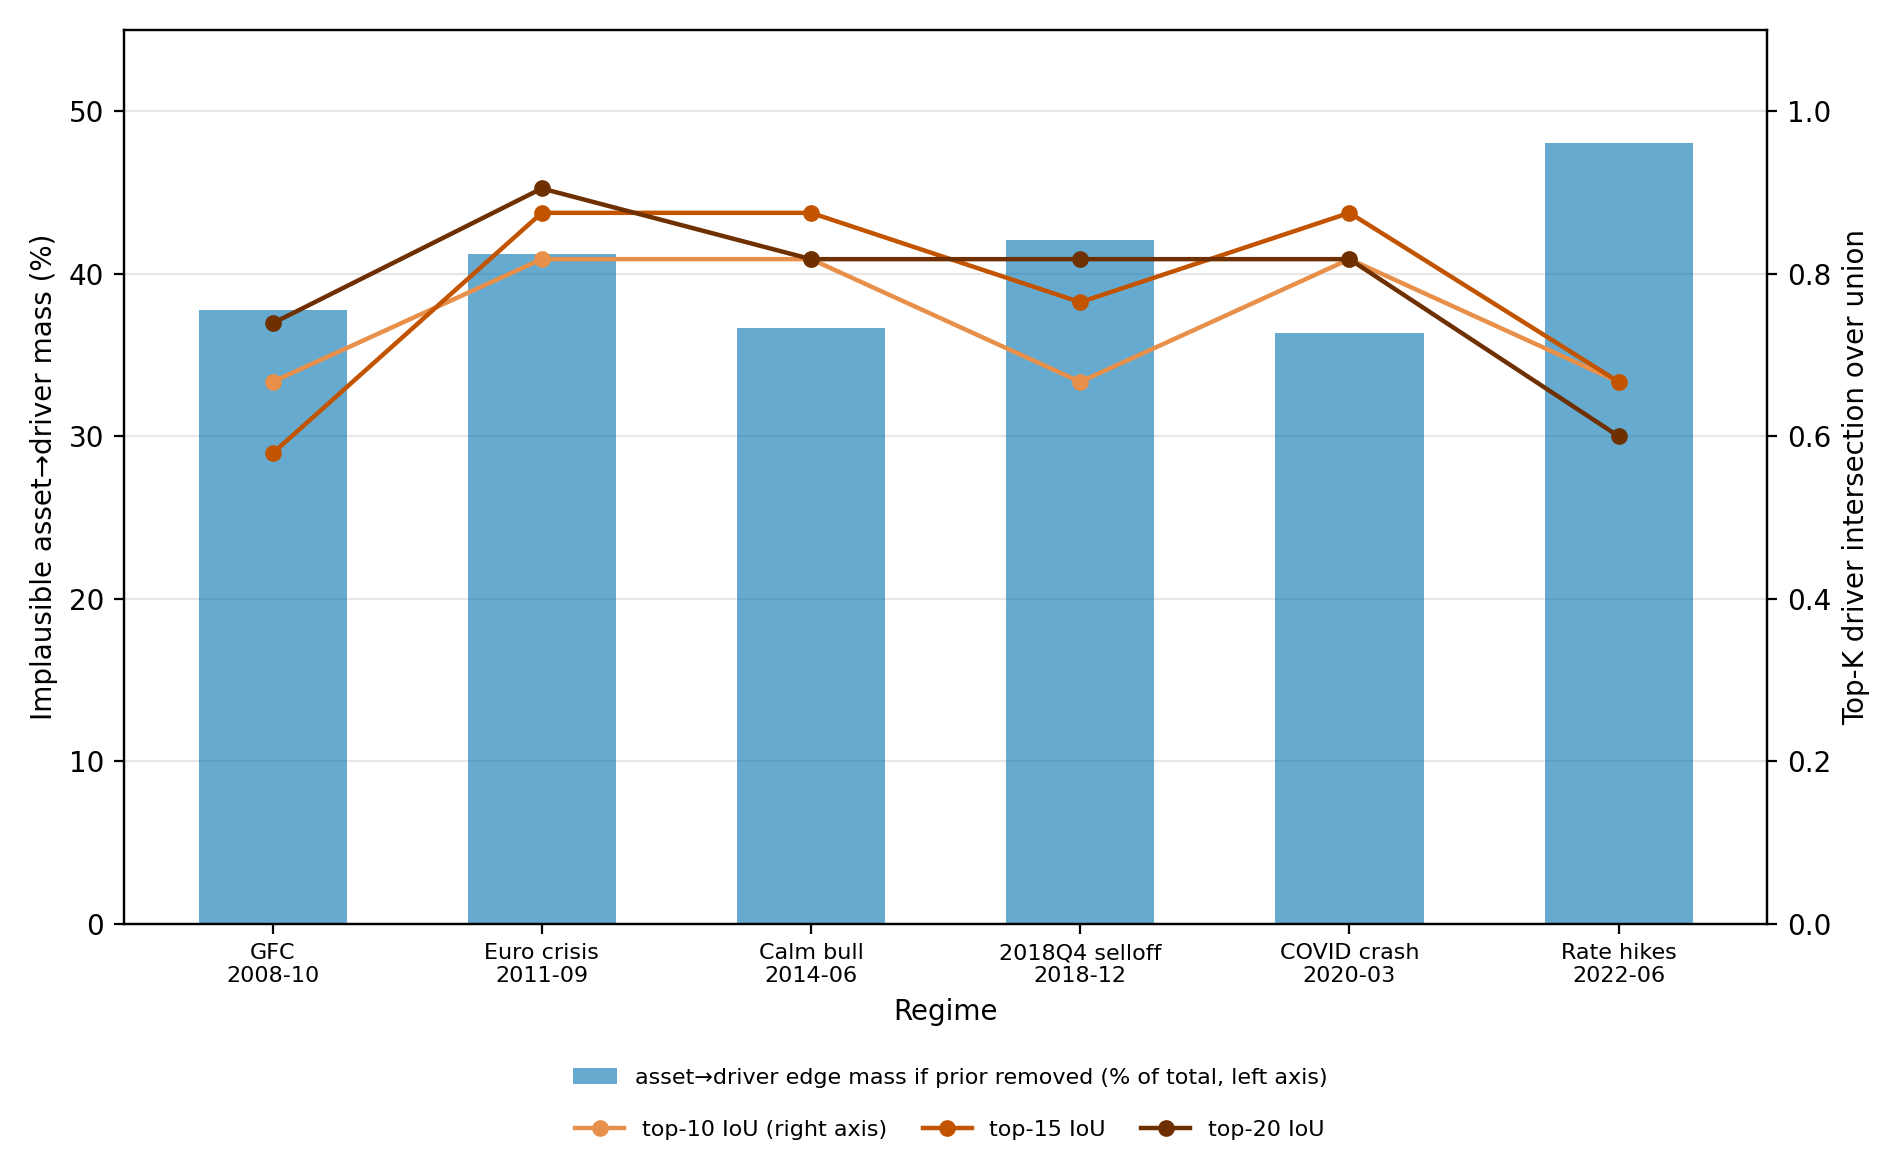
\includegraphics[width=0.92\textwidth]{figures/directional_prior.png}
  \caption{Verification of the asset$\to$driver directional prior. Bars: the
    fraction of total DYNOTEARS edge mass that would fall on implausible
    asset$\to$driver edges if the prior were removed (35--48\% across regime
    windows). Line (right axis): Jaccard overlap of the top drivers by
    edge mass with versus
    without the prior (a graph-content diagnostic). The prior removes a large block of spurious
    reverse-causation mass, and matters most in the 2008 and 2022 stress
    regimes.}
  \label{fig:prior}
\end{figure}

\section{The asset-graph chokepoint}
\label{sec:asset-graph}

The fixed-graph ablation is only valid if every allocator sees the
identical graph, so extraction is centralised in a single
chokepoint rather than left to each allocator. Per rebalance it reads the
asset--asset block $M$ of the fitted contemporaneous matrix; restricts rows
and columns together to the eligible universe at that date (so
late-inception names can never desynchronise the graph from the returns
panel); applies the magnitude threshold $\tau$ (default $0$; swept in the
sparsity-robustness analysis); and verifies acyclicity (a sub-block of a DAG
is a DAG). It also computes the per-asset structural residual variances on
the fit window (needed by the SEM-implied covariance of
Section~\ref{sec:d-family}) using the window's stored $z$-statistics, so
the residuals correspond exactly to the data the graph was fitted on.

\paragraph{What the graphs look like.} The DAGs are far from degenerate,
and stably so across estimation windows: at every length from 189 to 504
days the DYNOTEARS asset graphs average ${\sim}614$--$673$ directed edges
(density $6.3$--$6.9\%$ of possible ordered pairs) with a mean longest
directed
path of ${\approx}50$ nodes out of 99, indicating deep chains of influence
rather than a shallow hub-and-spoke structure. The graphs therefore contain
substantial orientation structure for the treatment allocators to exploit;
whatever the evaluation finds, it will not be attributable to trivially
symmetric graphs. One diagnostic is absent: month-to-month edge
persistence was not quantified
(Section~\ref{sec:limitations}). (The
same diagnostic flags a comparator limitation: VARLiNGAM's unpruned $B_0$
saturates to $32\%$ density at the 189-day window ($n=189$ observations
against $d=132$ variables), where DYNOTEARS' $\ell_1$ objective holds
density steady.)

\paragraph{What ``credible'' can mean without ground truth.} One objection
must be addressed directly: no true causal graph of the market is
available, so the
discovered graphs cannot be scored against an answer key. The pipeline is
therefore validated on everything that can be checked: the
directional prior has a quantified effect (above); the graphs are
structurally non-degenerate, with depth for the treatments to
exploit; discovery is deterministic, so the graphs are stable
facts about the data rather than artefacts of a run; disagreement between
discovery methods is retained as a diagnostic rather than averaged away
(Section~\ref{sec:comparators}); and, most importantly, the graphs are
judged by the controlled downstream ablation of
Chapters~\ref{chap:sensitivity}--\ref{chap:evaluation}, a task-based
test, which is the only economically meaningful one. The report accordingly
claims that the graphs are useful and reproducible, not that they
are true.

\section{Controls on the orientation content}
\label{sec:comparators}

Because the research question hinges on what the orientations contribute, the design
carries two further graph sources that perturb precisely that ingredient;
both feed the same chokepoint, so every allocator runs unchanged on them.
VARLiNGAM \cite{hyvarinen2010varlingam} supplies
differently-identified orientations: its instantaneous matrix $B_0$
is identified through non-Gaussianity rather than a score, LiNGAM's causal
order makes the asset block a DAG by construction, and its identification
assumption (heavy-tailed residuals) weakens mechanically at longer
windows, the window-fragility Chapter~\ref{chap:background} anticipated and
Chapter~\ref{chap:evaluation} observes. ridge-Granger supplies
magnitude-degraded orientations: a ridge-regularised VAR(1) on the
asset panel, in closed form, with
$M[i,j] = |{\rm coef}(x_{i,t-1}\!\to\!x_{j,t})|$, thresholded per window
to match the paired DYNOTEARS graph's edge density so the comparison is at
like-for-like sparsity. Its lagged, shrunken coefficients still order the
assets directionally, but they are not structural effect sizes, and it
is not guaranteed acyclic, which the allocators handle explicitly
(truncated-Neumann total effects; minimal feedback-arc removal before
topological ordering). The two controls therefore split ``orientation''
into its parts: if an effect needs DYNOTEARS' specific arrows, VARLiNGAM
should not reproduce it; if it needs trustworthy edge magnitudes
rather than arrows alone, ridge-Granger's ordering should survive where its
shock propagation fails, which is the dissociation
Section~\ref{sec:decomposition} observes. (A non-linear extension,
NTS-NOTEARS \cite{sun2023ntsnotears}, was probed at reduced scale and
is left as future work; Section~\ref{sec:future}.)

\section{Engineering for tractability and reproducibility}
\label{sec:cache}

Two engineering results underwrite the credibility of every number in
Chapter~\ref{chap:evaluation}.

\paragraph{The discovery cache.} The graph fit is the dominant cost
(${\approx}4$ minutes per window at $d\approx132$; ${\approx}15$ hours
per backtest), yet it depends only on the window data and discovery
hyperparameters, not on anything downstream. A content-keyed disk cache
therefore lets every configuration at a given window reuse one fit: the
full ablation grid ran against 1{,}684 cached graph fits with a
verified 100\% hit rate and zero refits, at ${\approx}40$ seconds per
backtest. The cache also guarantees the ablation's premise: allocators
cannot see different graphs, because there is exactly one graph per
(method, window, data) key. The cache mechanics are recorded in
Appendix~\ref{app:tables}.

\paragraph{A data-determinism defect, found and fixed.} Building the cache
exposed a latent reproducibility bug: one driver series (the
emerging-markets ETF EEM) was silently re-downloaded on every call, and
the resulting micro-jitter, amplified by the non-convex DYNOTEARS
optimiser, made the pipeline irreproducible at the bit level. Two
conclusions previously drawn in the project's first phase did not
survive the fix. (That first phase, an exploratory precursor on the
same panel and protocol, evaluated earlier causal allocators including
the skeleton variant this study anchors on; its configurations are
priced into the \rsNtrials-trial deflation universe of
Chapter~\ref{chap:evaluation}, and its committed skeleton result is the
target of the replication gate below.) All numbers in this report come
from the corrected, deterministic pipeline: two independent runs now
produce identical windows, weights and NAVs, verified end-to-end by the
replication gate of Section~\ref{sec:ablation-design}. A result that does
not survive a determinism fix was never real; treating reproducibility as a
prerequisite rather than an afterthought is part of the method
\cite{lopezdeprado2023causal}. The defect's mechanism, and the
observation that VARLiNGAM's ICA-based fits were robust to the same
jitter, are recorded in Appendix~\ref{app:tables}.
% ===== chapters/04_sensitivity.tex =====
% ============================================================
\chapter{From Graph to Weights}
\label{chap:sensitivity}
% ============================================================

This chapter addresses the challenge of using direction at all. Hierarchical
allocators consume a symmetric distance, symmetrisation discards the
orientations, and there is no established way to feed an asymmetric DAG
adjacency into clustering or risk allocation. The deliverable is the
allocation machinery that makes the research question answerable: an
orientation-aware allocator family fed the identical per-window graph, split
into orientation-blind controls that can see only the skeleton and treatments
that can see the orientations, assembled into a fixed-graph ablation in which
orientation is the only treatment variable. The family is the construction that
discharges
Premise 2: without it, the value of orientation cannot be measured at
all. Section~\ref{sec:symm} states the problem;
Section~\ref{sec:sem} derives the structural quantities the treatments
consume; Sections~\ref{sec:controls}--\ref{sec:d-family} define the
allocators; and Section~\ref{sec:ablation-design} assembles them into the
fixed-graph ablation.

\section{The symmetric-clustering problem}
\label{sec:symm}

Hierarchical allocation (Section~\ref{sec:hrp-theme}) consumes a symmetric,
non-negative distance matrix; a causal graph is asymmetric by design, and
this asymmetry is the object of study. The naive fix, symmetrising the
adjacency as
$\tfrac{1}{2}(|M| + |M^\top|)$, discards the very orientations the research
question asks
about. A more principled alternative, embedding the directed matrix
losslessly in the symmetric bipartite double cover, was investigated
and abandoned: it doubles the node set into source and sink roles, and
recombining each asset's two role-weights into one holding re-poses
precisely the upstream-versus-downstream question the construction was
meant to absorb. That failure sets the design conclusion for the
chapter: the
symmetric interface cannot be made to carry orientation, so the
allocation steps themselves must change. The challenge is therefore not to
force $M$ into the existing
interface but to build allocation steps that consume the directed
matrix natively, while changing as little else as possible, so that any
performance difference is attributable to orientation and nothing else. The
two structural observations of Section~\ref{sec:hrp-theme} open the way.
First, HRP's dendrogram exists only to produce a leaf ordering for
recursive bisection, and a DAG carries a natural ordering for free.
Second, HRP's bisection step consumes cluster variances from a
covariance matrix, and a DAG implies one.

\section{The structural model: total effects and the implied covariance}
\label{sec:sem}

Both DYNOTEARS' $W$ and VARLiNGAM's $B_0$, restricted to the asset block and
written in the $i\to j$ convention, define the structural equation model
\begin{equation}
  (I - M^\top)\, x = \varepsilon
  \qquad\Longrightarrow\qquad
  x = (I - M^\top)^{-1} \varepsilon \;=:\; B\,\varepsilon,
  \label{eq:sem}
\end{equation}
where $x$ is the vector of (standardised) asset returns and $\varepsilon$ the
vector of structural shocks. Because the asset block is a DAG, its adjacency
is nilpotent, so the total-effect matrix
$B = \sum_{k\ge 0} (M^\top)^k$ terminates in at most $N$ terms and exists
exactly, with no spectral-radius assumption. $B_{ij} = \partial x_i / \partial
\varepsilon_j$ aggregates the influence of a unit shock at asset $j$ on asset
$i$ over all directed paths; it is the Leontief inverse of
input--output economics, and its asymmetry is where orientation enters
allocation natively. (For the non-DAG ridge-Granger control, $B$ is approximated
by the truncated series with a spectral-radius guard, a documented
approximation.)

The SEM of Eq.~\eqref{eq:sem} implies a covariance. With $\Sigma_\varepsilon =
\operatorname{diag}(\sigma^2_{\varepsilon,i})$ (diagonality is the SEM's
own independent-shocks assumption, and estimating a dense
$\Sigma_\varepsilon$ would reintroduce sample correlation into a treatment
meant to isolate the graph), the SEM-implied covariance in return
units is
\begin{equation}
  \Sigma_{\mathrm{SEM}}
  \;=\; D_\sigma \big( B\, \Sigma_\varepsilon\, B^\top \big) D_\sigma ,
  \label{eq:sigma-sem}
\end{equation}
where the shock variances are estimated from the fit window's structural
residuals $E = X_z (I - M)$, and $D_\sigma$ de-standardises from the
$z$-scored units the graph was fitted in back to return units. The name
merits precision: $\Sigma_{\mathrm{SEM}}$ is the covariance of the
observables that the structural model implies (SEM's $\Sigma(\theta)$,
the reduced form in SVAR terms), whereas the structural shocks' own
covariance is the diagonal $\Sigma_\varepsilon$ above. The
de-standardisation is not optional: recursive bisection compares cluster
variances, and omitting $D_\sigma$ would silently equalise asset
volatilities. Two caveats are stated rather than hidden: the asset-block SEM
marginalises over the drivers, so $\varepsilon$ absorbs driver-explained
variance and its diagonality is an approximation; and
$\Sigma_{\mathrm{SEM}}$ is projected to the nearest positive semi-definite
(PSD) matrix and lightly ridge-loaded
so dense stress-window graphs cannot produce a singular input.

\section{The controls: correlation and skeleton}
\label{sec:controls}

\paragraph{\HRP{} (the correlation control).} Textbook HRP
\cite{lopezdeprado2016hrp}: the distance $\sqrt{\tfrac{1}{2}(1-\rho_{ij})}$
on the
lookback window's sample correlation, with the sample covariance for
bisection. It is
graph-blind (verified by unit test: changing the graph cannot change its
weights) and anchors the decomposition.

\paragraph{\skelsamp{} (the skeleton control).} The graph replaces the
correlation matrix,
but symmetrically: each asset is embedded by its edge profile
$e_i = [\,M_{i\cdot},\, M_{\cdot i}\,]$ and the clustering distance is
$D_{ij} = \lVert e_i - e_j \rVert_2$, with the sample covariance for
bisection.
This embedding is provably invariant to global orientation reversal:
transposing $M$
(reversing every edge) swaps the two halves of every $e_i$, leaving all
pairwise distances, and hence the dendrogram and the weights, unchanged;
the property is enforced by unit test. The guarantee is exactly that and
no more: because $e_i$ keeps outgoing and incoming edges in separate
halves, reversing an individual edge can move mass between halves
and change distances, so \skelsamp{} retains each asset's source/sink
role profile, which is information the undirected skeleton alone does not
carry. The control with the stronger guarantee is \skelalt{} below, and
the decomposition is read against both anchors in
Chapter~\ref{chap:evaluation}. \skelsamp{} coincides with
the skeleton allocator evaluated in the project's first phase
(Section~\ref{sec:cache}), which allows the
new harness to be validated against a
committed historical result (Section~\ref{sec:ablation-design}).

\paragraph{\skelalt{} (a second symmetrisation).} Hierarchical clustering
demands
a symmetric distance and $M$ is not symmetric, so building a skeleton
control
requires choosing a symmetrisation, and the choice is not unique. If
the skeleton's measured contribution depended on which one was made, it
would be a fact about the
recipe rather than about the skeleton. \skelalt{} is a control on the
control: the
same pipeline, but with the $\tfrac{1}{2}(|M|+|M^\top|)$ distance, so that
two
assets are close when a strong link joins them rather than when their
edge profiles match. Of the two, \skelalt{} carries the stronger
orientation-blindness guarantee: $\tfrac{1}{2}(|M|+|M^\top|)$ is a
function of the undirected weighted adjacency alone, hence invariant to
reversing any single edge, where \skelsamp{}'s embedding is invariant
only to reversing all of them at once. Comparing them
tests whether ``the skeleton'' has been
identified accidentally with one particular symmetrisation, and
Chapter~\ref{chap:evaluation} reports where the two anchors disagree.

\section{The orientation-aware family}
\label{sec:d-family}

Section~\ref{sec:symm} left hierarchical allocation with exactly two moving
parts, and that fact bounds the design space. The clustering step exists only
to emit an ordering; the allocation step consumes only a
covariance. Nothing else crosses between them: recursive bisection
receives the ordering and the covariance and no third object, and it splits
the ordered list by position rather than by the dendrogram's own branches. A
causal graph therefore has exactly two entry points into HRP, the ordering
and the covariance, and crossing them
enumerates the family completely (Table~\ref{tab:crossing}).

\begin{table}[h]
  \centering
  \caption{The two entry points, crossed. The row is where the ordering
    comes from,
    the column is what recursive bisection splits on; \skelsamp{} is the
    control that takes orientation through neither.}
  \label{tab:crossing}
  \begin{tabular}{l l l}
    \toprule
    Ordering from & splits on sample cov. & splits on $\Sigma_{\mathrm{SEM}}$ \\
    \midrule
    clustering on the skeleton & \skelsamp{} (control) & \skelsem{} \\
    topological sort           & \orientsamp{}           & \orientsem{} \\
    \bottomrule
  \end{tabular}
\end{table}

Two points about the rows follow. The first row keeps the clustering step
and feeds
it a graph-derived distance; the second removes the clustering step
entirely, because a DAG already carries an ordering and needs no dendrogram
to produce one. What distinguishes the rows is therefore ``where the
ordering comes from'', not
``what the clustering step reads''. Each treatment differs from the
control in exactly one respect (\skelsem{} in the covariance alone,
\orientsamp{} in the
ordering alone, \orientsem{} in both), so the results chapter can localise
not just
whether orientation carries value but where. All three are long-only,
fully invested, deterministic and seed-free; all take the identical
$(M,\ \text{returns window})$ inputs as the controls; none has an analogue in
the hierarchical-allocation literature.

\paragraph{\skelsem{} (SEM-implied covariance).} Clustering is as in
\skelsamp{}: the
ordering is deliberately held at the skeleton, so that
$\skelsem{}-\skelsamp{}$ isolates orientation's effect on the allocation
step
alone. Recursive bisection, however, allocates on $\Sigma_{\mathrm{SEM}}$
of
Eq.~\eqref{eq:sigma-sem} instead of the sample covariance: orientation
enters through the shock-propagation asymmetry of $B$.

\paragraph{\orientsamp{} / \orientsem{} (causal-ordered bisection).}
\label{sec:d2}
The clustering step is removed entirely. HRP's dendrogram exists only to
produce a quasi-diagonalising leaf order, and a DAG supplies an order
natively: assets are sorted upstream$\to$downstream by a topological sort
of
$M$ (ties broken deterministically by total downstream influence
$\sum_r |B_{ri}|$, then name), and the existing recursive bisection
runs on that order, with the sample covariance (\orientsamp{}) or with
$\Sigma_{\mathrm{SEM}}$ (\orientsem{}). This is the most direct response
to the
observation that one cannot cluster on an asymmetric matrix: do not
cluster.
One subtlety, identified by the ablation's own tests, should be recorded:
recursive bisection is mirror-invariant (reversing the leaf order
reproduces the identical partition tree), so \orientsamp{} responds to
orientation
through the partition structure the order induces, not through the
upstream/downstream direction itself.

\section{The fixed-graph ablation}
\label{sec:ablation-design}

The experimental design is what turns the family into an answer to the research
question.

\paragraph{Design.} At every rebalance the chokepoint
(Section~\ref{sec:asset-graph}) hands the identical graph $M$ to
every allocator in Table~\ref{tab:variants}; everything else (universe,
calendar, costs,
covariance-estimation window, and allocator internals downstream of the
distance/
covariance/ordering choice) is shared code. Orientation is therefore the
sole treatment variable, and the decomposition is two differences with a
common anchor: $\skelsamp{}-\HRP{}$ (skeleton) and
$\orientany{}-\skelsamp{}$ (orientation). The shared anchor cancels when
the two are added,
$(\skelsamp{}-\HRP{}) + (\orientany{}-\skelsamp{}) =
\orientany{}-\HRP{}$, so the total causal-graph gain is attributed
without remainder. The reported grid is five graph-consuming allocators $\times$
\{DYNOTEARS, VARLiNGAM\} $\times$ \{189, 252, 378, 504\}-day windows, plus
the magnitude-degraded ridge-Granger control arm, a sparsity sweep and a cost
sweep. The evaluated grid is wider: seven allocators in the original
experiment plan, plus the mechanism controls (two direction-free
covariance controls and a graph-free partial-correlation skeleton
control), a second hierarchical family (HERC) and the naive anchors,
all added during
evaluation; the narrowing to five and the provenance of every extension
are disclosed in Section~\ref{sec:believe}, and every evaluated cell is
priced into the deflation universe. The window axis is a
design variable in its own right: the sample moments every allocator
consumes degrade in opposite directions as the window shrinks (estimation
noise) or grows (staleness across regimes), so tracing the decomposition
over estimation windows from nine months to two years tests where each kind of
graph information adds value. Every cell of the grid is reported. At the
shortest window the discovery
fit
operates with $n=189$ observations against $d=132$ variables: valid
($n>d$) but thin, a caveat carried through to the results.

\paragraph{Verification before results.} Three gates preceded the grid.
The unit-test gate: 60+ tests written first, including the
orientation-blindness of the controls, the orientation-sensitivity of every
treatment, total-effect and SEM-covariance identities against
hand-computed cases, and topological-order properties on random
DAGs. The cache gate: every graph fit verified
as a cache hit with zero refits, so no allocator can have seen a different
graph. The replication gate: \skelsamp{} run through the new
harness exactly reproduces
the committed first-phase bundle, establishing both that the new
machinery is faithful and that
the pipeline is deterministic end-to-end. The gates' figures are
archived in Appendix~\ref{app:tables}.

\begin{table}[t]
  \centering
  \caption{The allocator family. All share
    the universe, calendar, transaction costs and rebalance schedule.}
  \label{tab:variants}
  \small
  \setlength{\tabcolsep}{4.5pt}
  \begin{tabular}{l l l l}
    \toprule
    Allocator & Ordering from & Bisection covariance & Reads orientation? \\
    \midrule
    \HRP{} & correlation distance & sample & no (graph-blind) \\
    \skelsamp{}            & graph embedding      & sample & no (transpose-inv.) \\
    \skelalt{}           & $\tfrac{1}{2}(|M|{+}|M^\top|)$ & sample & no (per-edge inv.) \\
    \skelsem{}            & graph embedding      & $\Sigma_{\mathrm{SEM}}$ & allocation step \\
    \orientsamp{}            & topological order    & sample & ordering step \\
    \orientsem{}           & topological order    & $\Sigma_{\mathrm{SEM}}$ & both steps \\
    \bottomrule
  \end{tabular}
\end{table}
% ===== chapters/05_evaluation.tex =====
% ============================================================
\chapter{Decomposing the Gain}
\label{chap:evaluation}
% ============================================================

This chapter addresses the challenge of inference at realistic effect sizes.
The effects at stake are of the order of 0.01 to 0.03 Sharpe on about
18 years of data, spread across many evaluated configurations, and a
pairwise $p$-value means nothing there without pricing the multiplicity,
quantifying the power and controlling for non-causal mechanisms such as
shrinkage and market-factor removal. The deliverable is a pre-registered,
controlled, multiplicity-aware evaluation: block bootstrap, deflated Sharpe,
SPA and MCS including a pooled SPA, a minimum detectable effect,
pre-committed controls and an out-of-sample slice. Its structure follows the
logical order in which the research question must be answered. Section~\ref{sec:method} fixes
how the gain is measured. Section~\ref{sec:r1} tests Premise 1,
whether the causal graph improves on the correlation matrix at all.
Section~\ref{sec:decomposition} presents the decomposition of the gain
into
skeleton and orientation (the answer to the research question), together with its
robustness to the design's free parameters. Section~\ref{sec:believe-rigour}
subjects every claim to the multiplicity-aware inference battery, and
Section~\ref{sec:believe} closes with the threats to validity.

\section{Measurement protocol}
\label{sec:method}

\paragraph{Protocol.} Every configuration runs the identical walk-forward
backtest: the fixed 99-name universe, monthly rebalancing over 2007--2024
(215 rebalances at windows up to one year; the 18-month and two-year
windows' longer burn-ins leave 209 and 203), estimation windows of 189, 252,
378 and 504 trading days for both the graph fit and the sample covariance,
weights held for 21 trading days, transaction costs of 5\,bps per unit of
one-way turnover (swept over $\{0,5,10,20\}$\,bps). ``Performance'' always means the out-of-sample,
net-of-cost, annualised Sharpe ratio of daily portfolio returns, reported
alongside CAGR, maximum drawdown and mean turnover
(Table~\ref{tab:return-terms} in Appendix~\ref{app:tables} tabulates them
for the headline
configurations); no in-sample number appears anywhere in this report, and
gross figures appear only as the zero-cost arm of the cost sweep.

\paragraph{Inference.} Pairwise contrasts use the Politis--Romano stationary
block bootstrap \cite{politis1994stationary} (10{,}000 resamples, mean
block 21
days), which resamples the joint return panel so cross-strategy correlation
is preserved. Because daily returns here are heavily non-normal (excess
kurtosis ${\approx}\,\rsKurtosis$; Figure~\ref{fig:retdist},
Appendix~\ref{app:tables}) and because this
project evaluated \rsNtrials\ configurations in total (the deflation
universe deliberately keeps byte-identical duplicates, a conservative
choice), pairwise
$p$-values are never taken at face value: every claim is re-adjudicated by
the battery of Section~\ref{sec:believe-rigour}: Probabilistic and
Deflated Sharpe ratios \cite{bailey2012psr,bailey2014deflated} (the DSR
deflating against all \rsNtrials\ trials), Hansen's SPA
\cite{hansen2005spa}, the studentised successor of White's Reality
Check \cite{white2000reality}, for each
family-wise comparison, and the $90\%$ Model Confidence Set
\cite{hansen2011mcs}. Regimes are defined by NBER recession dates and
top/bottom VIX quintiles.

\paragraph{Stability.} Every allocator in the study is deterministic and
seed-free: two independent end-to-end runs produce identical graphs,
weights and NAVs, a property verified by the replication gate
(Section~\ref{sec:ablation-design}). Every number in this chapter comes
from the pipeline of Section~\ref{sec:cache}.

\section{Premise 1: the causal graph against the correlation matrix}
\label{sec:r1}

Premise 1 asks whether there is any gain to decompose. The like-for-like
comparison is the graph-blind \HRP{} control against the causal-graph
allocators on the same machinery, at all four windows. The control itself
earns $\rsCorrSharpeWone$, $\rsCorrSharpe$, $\rsCorrSharpeWthree$ and
$\rsCorrSharpeWfive$ at the 189-, 252-, 378- and 504-day windows; the
decomposition's reference treatment (\skelsem{}, which differs from the
skeleton control in the allocation step alone) delivers a total
causal-graph gain over it of $+0.018$,
$+0.031$, $+0.030$ and $+0.032$ respectively ($p=0.43$--$0.11$;
Table~\ref{tab:decomp}), with \orientsem{} reaching $+0.036$ at two
years. Of the 40
graph-versus-\HRP{} cells (five graph-consuming allocators, both
discovery methods, four windows), 36 are above the control (19 of 20 under
DYNOTEARS; the single exception is the skeleton-only allocator at the
nine-month window). This consistency should be read as robustness, not as
significance: the cells share one return panel, overlapping windows and
common machinery, so they are far from independent draws and no sign-count
converts into a valid $p$-value. What it establishes is that the gain's
direction does not depend on the choice of allocator, discovery method or
window; no cell is individually significant, and inference under the
panel's dependence structure is delegated to the family-wise tests of
Section~\ref{sec:believe-rigour}. In brief: Hansen's SPA rejects
nowhere over the full allocator grid, and crosses the $5\%$ bar only at
the two longest windows under a narrowed family fixed after these
results were seen. Premise 1 therefore rests on the sign
consistency and the stable total, not on family-wise significance: the
causal graph out-performs the correlation matrix by a modest margin at
every window. The decomposition that follows
does not stand or fall with Premise 1 in any case: it compares the
graph-fed allocators against each other on identical inputs, so it
remains informative about where any gain, whatever its size, comes
from. In return
terms the gain is $+0.4$ to $+0.7$ percentage points of net CAGR per year
($5.62\%$ vs $4.97\%$ for \skelsem{} against the control at one year;
Table~\ref{tab:return-terms}). Two naive anchors bound the absolute
levels: equal weight earns $\rsEwSharpe$ and inverse variance
$\rsIvpSharpe$ at one year (Table~\ref{tab:return-terms}), so every
member of the hierarchical family clears $1/N$ at every window, though
the correlation control itself trails inverse variance at three of the
four windows. The
thesis's claims are contrasts within the family; the anchors size the
family's absolute edge on this universe as modest.

\section{The decomposition: skeleton versus orientation}
\label{sec:decomposition}

\subsection{The decomposition across estimation windows}

Figure~\ref{fig:gradient} is the thesis's central result:
the two components of the decomposition traced across the four estimation
windows. Table~\ref{tab:decomp} gives the numbers,
Figure~\ref{fig:heatmap} the full
allocator--method matrix, and Figure~\ref{fig:decomp}
(Appendix~\ref{app:tables}) the per-window levels. Three features carry the answer to the research
question. First, the
total causal-graph gain is stable: $+0.018$ to $+0.032$ (\skelsem{}) at
every
estimation window, rising to $+0.036$ for \orientsem{} at two years. Second, the
skeleton contribution is hump-shaped ($-0.003$ at nine months, peaking at
$+0.022$ at the one-year convention, decaying to $+0.009$ at two years) and
never individually significant ($p \geq 0.14$). Third, the
orientation contribution is positive at every window and U-shaped ($+0.021$ at
$p=0.08$, $+0.009$ at $p=0.45$, $+0.012$ at $p=0.31$, $+0.023$ at
$p=0.048$): largest at the two extremes, smallest where the skeleton peaks,
with 11 of the 12 DYNOTEARS orientation contrasts positive across the grid
(Figure~\ref{fig:forest}). The two components are roughly complementary,
which is why the total is flat while its composition shifts. Family-wise,
the direction-aware variants against the shared skeleton control reject
only at two years, where the pairwise effect also peaks, and only under
the narrowed family; Section~\ref{sec:believe-rigour} reports both
families and sizes that rejection.

\paragraph{Anchor-dependence of the shapes.} The contributions above are
anchored
on \skelsamp{}. Re-anchoring on \skelalt{}, the symmetrisation with the
stronger orientation-blindness guarantee (Section~\ref{sec:controls}),
changes them: the skeleton contribution becomes flat ($+0.022$, $+0.018$,
$+0.024$, $+0.019$ across the four windows) and the orientation
contribution
becomes $-0.003$/$+0.013$/$+0.006$/$+0.012$ for \skelsem{}
($-0.003$/$+0.008$/$+0.010$/$+0.016$ for \orientsem{}; point estimates,
not formally tested). The two anchors agree that orientation's increment
is positive at every window from one year out and largest at the longer
estimation windows; they disagree at nine months, where \skelalt{}
beats \skelsamp{} by $+0.025$ ($p=0.013$), the strongest
control-versus-control divergence in the study. At the shortest window
the choice of symmetrisation therefore matters as much as orientation
itself, and the nine-month column is read with that caveat throughout.
The hump and the U are \skelsamp{}-anchored
descriptions; the anchor-robust findings are the flat-to-positive
skeleton gain and the orientation increment at long estimation windows.

\begin{figure}[tbp]
  \centering
  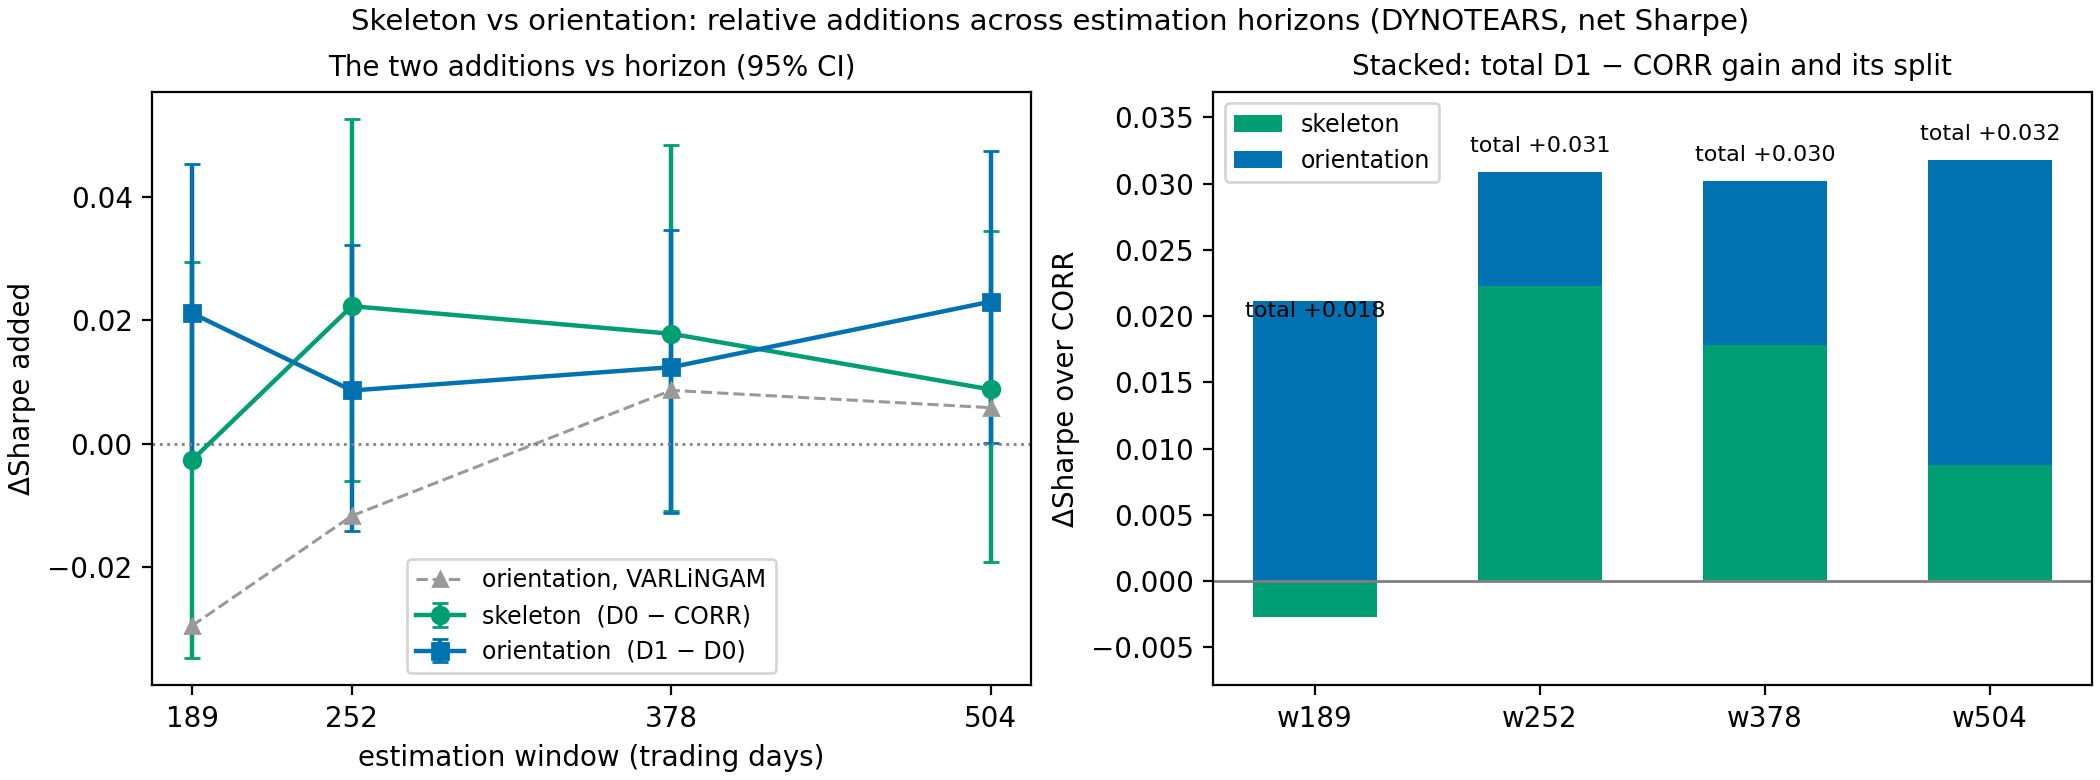
\includegraphics[width=0.99\textwidth]{figures/phase_ii_window_gradient.png}
  \caption{The central result: the two components of the decomposition as a
    function of estimation-window length (DYNOTEARS, net Sharpe). Left: the
    skeleton addition (\skelsamp{} $-$ \HRP{}, hump-shaped) and the
    orientation addition (\skelsem{} $-$ \skelsamp{}, U-shaped, positive throughout) with
    $95\%$ block-bootstrap CIs; the VARLiNGAM orientation series (grey)
    scatters around zero (mean $-0.005$), dipping below it at the
    nine-month window. Right: the same two additions stacked. The total gain
    is stable while its composition shifts, orientation contributing most
    where the sample moments feeding the control are weakest.}
  \label{fig:gradient}
\end{figure}

\begin{table}[t]
  \centering
  \caption{The decomposition (DYNOTEARS): pairwise $\Delta$Sharpe with
    Politis--Romano $p$-values at each estimation window. The total splits
    by the shared anchor: total $=$ skeleton $+$ orientation.}
  \label{tab:decomp}
  \small
  \setlength{\tabcolsep}{4pt}
  \begin{tabular}{l c c c c}
    \toprule
    & \multicolumn{4}{c}{Window (days)} \\
    \cmidrule(lr){2-5}
    Contrast & 189 & 252 & 378 & 504 \\
    \midrule
    skeleton: \skelsamp{} $-$ \HRP{} & $-0.003$ (0.85) & $+0.022$ (0.14) & $+0.018$ (0.24) & $+0.009$ (0.53) \\
    orientation, allocation step: \skelsem{} $-$ \skelsamp{}     & $+0.021$ (0.08) & $+0.009$ (0.45) & $+0.012$ (0.31) & $+0.023$ (0.048) \\
    orientation, both steps: \orientsem{} $-$ \skelsamp{}   & $+0.021$ (0.19) & $+0.003$ (0.82) & $+0.017$ (0.29) & $+0.027$ (0.057) \\
    \midrule
    total: \skelsem{} $-$ \HRP{}   & $+0.018$ (0.43) & $+0.031$ (0.15) & $+0.030$ (0.15) & $+0.032$ (0.11) \\
    total: \orientsem{} $-$ \HRP{} & $+0.019$ (0.42) & $+0.026$ (0.24) & $+0.035$ (0.10) & $+0.036$ (0.077) \\
    \bottomrule
  \end{tabular}
\end{table}

\begin{figure}[tbp]
  \centering
  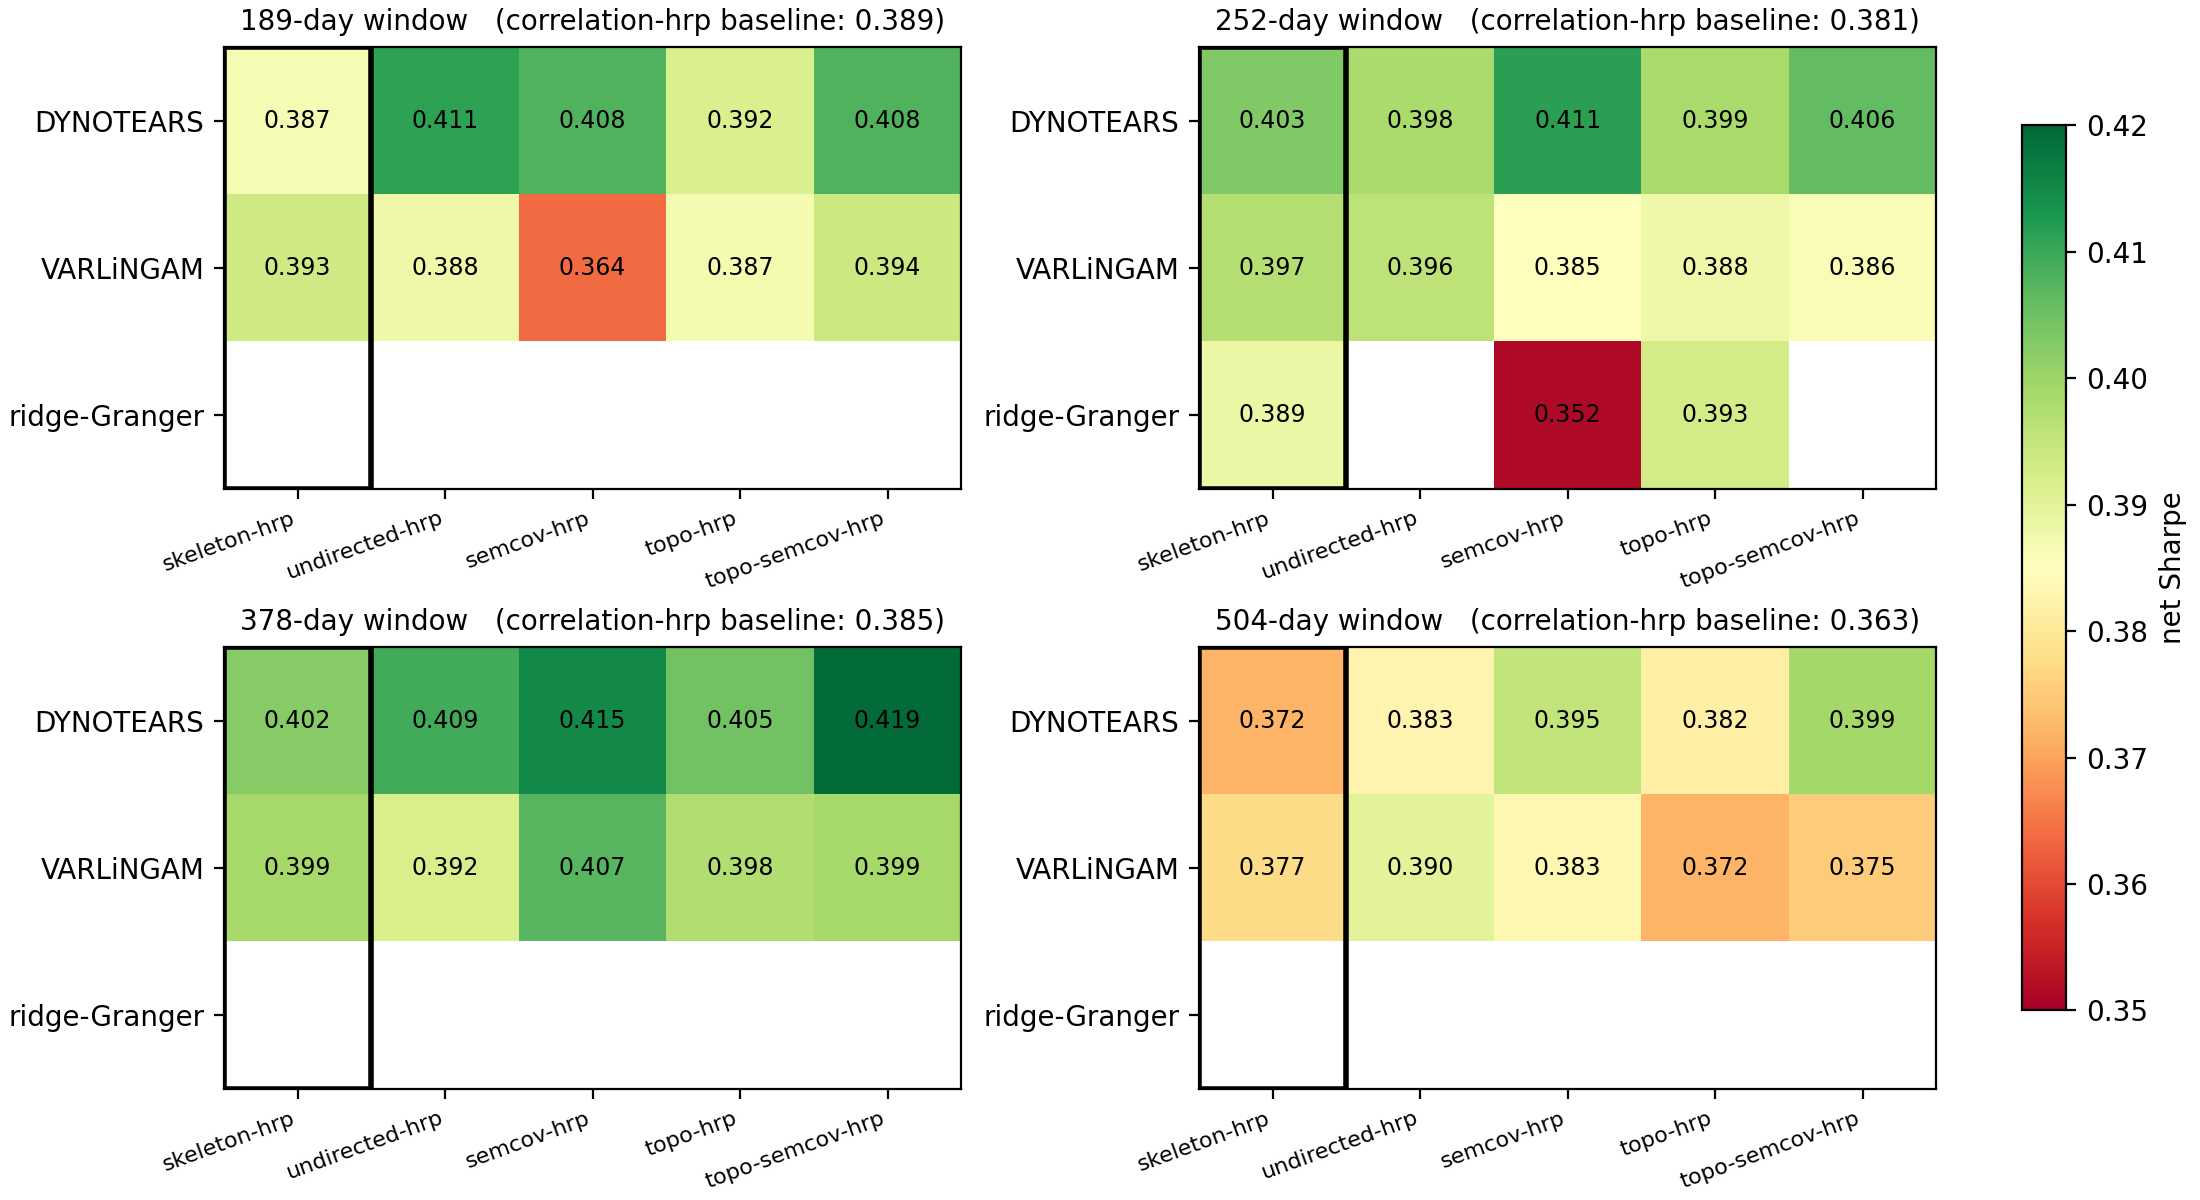
\includegraphics[width=0.99\textwidth]{figures/phase_ii_heatmap.png}
  \caption{Net Sharpe by discovery method $\times$ allocator at the four
    windows (boxed column: the symmetrised control \skelsamp{}; panel titles carry
    the \HRP{} baseline). The DYNOTEARS orientation-aware cells (\skelsem{},
    \orientsem{}) are strong at every window (\orientsem{} at 378 days,
    0.419, is the
    study-wide best), while the VARLiNGAM rows show no orientation effect
    anywhere.}
  \label{fig:heatmap}
\end{figure}

\begin{figure}[tbp]
  \centering
  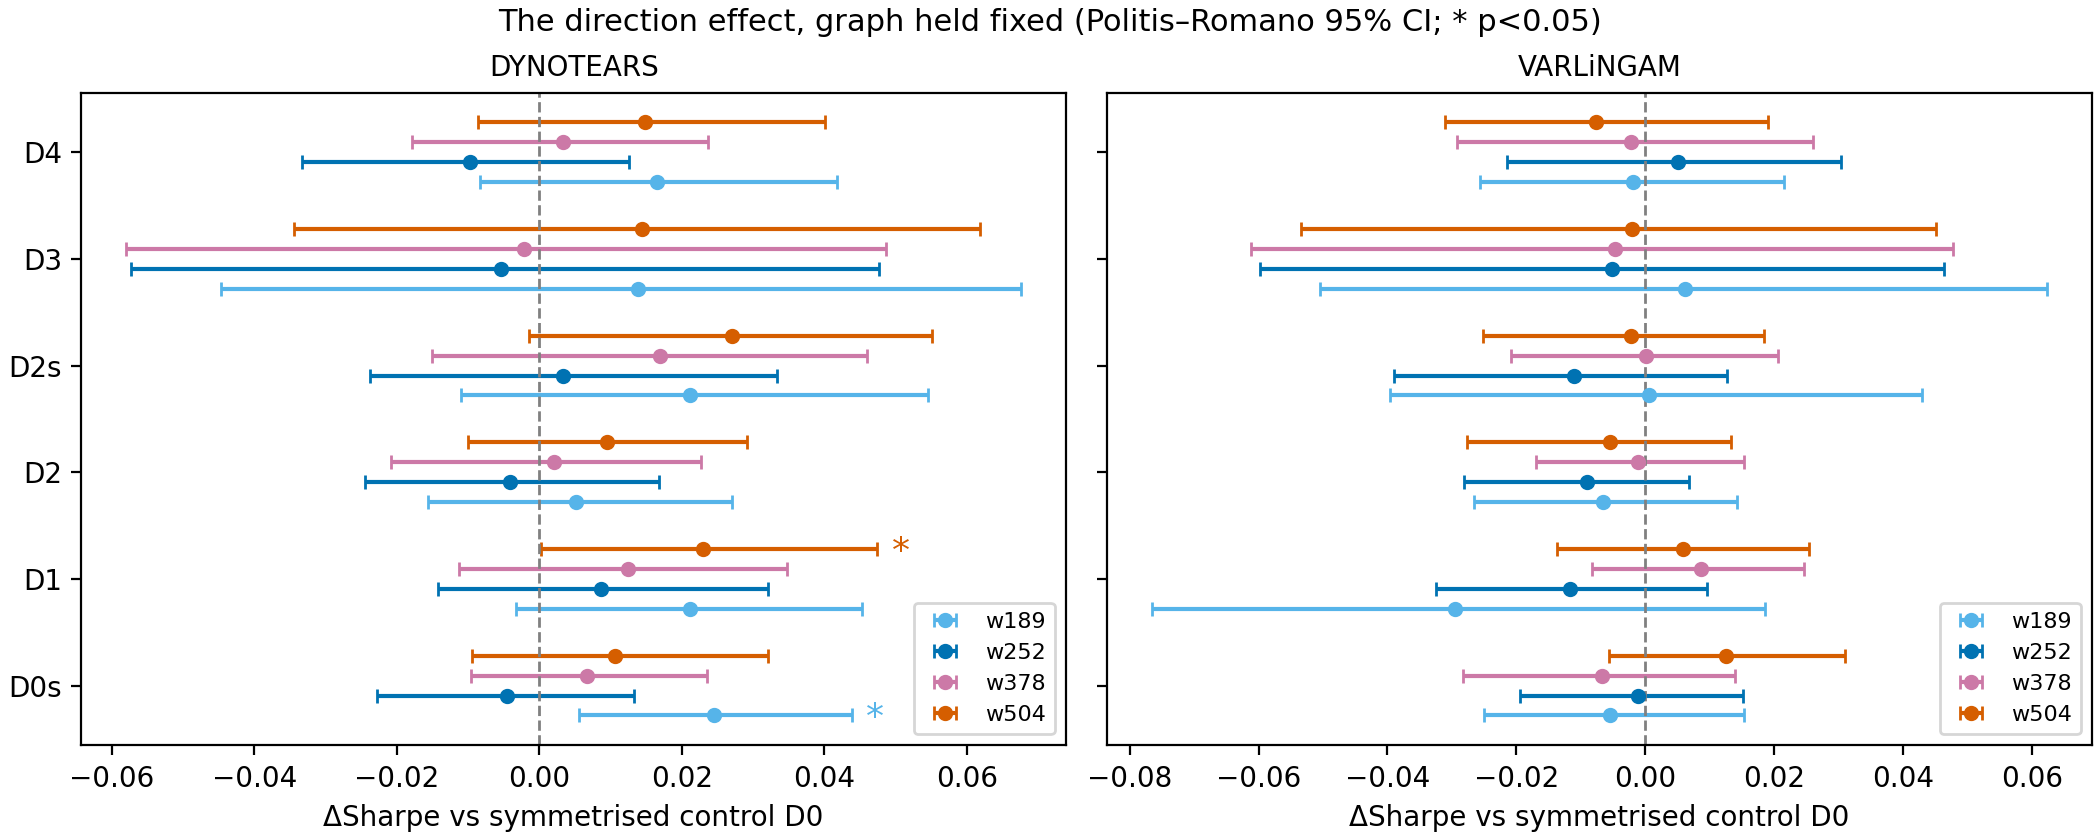
\includegraphics[width=0.99\textwidth]{figures/phase_ii_forest.png}
  \caption{The fixed-graph orientation effect: $\Delta$Sharpe of each
    orientation-aware allocator against the skeleton control \skelsamp{} at all four
    windows, with $95\%$ block-bootstrap CIs ($\ast$: $p<0.05$). Eleven of
    twelve DYNOTEARS contrasts are positive (\skelsem{} starred at two years); the
    VARLiNGAM contrasts scatter around zero (4/12 positive). The starred
    \skelalt{} cell at the nine-month window is a control-versus-control
    divergence, discussed in the text.}
  \label{fig:forest}
\end{figure}

\subsection{What orientation contributes}
\label{sec:orientation-role}

Orientation contributes robustness to the estimation window rather than
level. The skeleton
allocator's performance is window-fragile ($0.372$--$0.403$ across the four
windows, and below the control at nine months); \skelsem{}
($0.395$--$0.415$) and
\orientsem{} ($0.399$--$0.419$) are strong everywhere
(Figure~\ref{fig:nav} shows the
one-year NAV paths). The U-shape of Figure~\ref{fig:gradient} indicates
when orientation pays: when the sample moments
feeding the allocator are least reliable. At 189 days the sample covariance
is estimated from barely $1.9$ observations per asset (noise); at 504 days
it averages across regimes it should distinguish (staleness); and at the
one-year window, where the estimation literature puts the
noise--staleness optimum and where the skeleton's own contribution peaks,
orientation adds least. $\Sigma_{\mathrm{SEM}}$, built from the
contemporaneous graph and its shock variances, substitutes structure
for sample-moment quality at both ends of that trade-off. On this reading,
the SEM covariance acts as a regulariser of the allocation step rather
than a source of extra return; the controls at the end of this
subsection identify which of its properties does the regularising, and
the answer is not direction. Two qualifications bound the mechanism. First,
the window moves the graph and the sample moments together (both are
estimated on the same lookback), so the gradient cannot by itself
separate moment degradation from graph degradation; the stability of the
discovered graphs across windows (density $6.3$--$6.9\%$ at every
estimation window; Section~\ref{sec:asset-graph}) supports the
reading that the moments degrade faster. Second, the nine-month arm of
the U is anchor-dependent (Section~\ref{sec:decomposition}), so the
regulariser mechanism is claimed only for the long-window arm.

\paragraph{An alternative explanation, tested directly.} The
contrast $\skelsem{}-\skelsamp{}$ compares the SEM-implied covariance
against the sample covariance, and $\Sigma_{\mathrm{SEM}}$ differs from
the sample covariance in more ways than direction: it is a structured
estimator (fewer effective parameters, shrinkage-like in character), and
its independent-shock assumption strips out the common market component.
Either property is achievable with no graph at all, so a sceptic could
read the covariance-channel gain as generic shrinkage or as
de-factoring. I test both directly, with the interpretation of every
possible outcome written down and committed before either control was
run (Section~\ref{sec:believe}): the skeleton allocator's clustering is
kept fixed and its sample covariance is replaced by (i) a Ledoit--Wolf
shrunk covariance \cite{ledoitwolf2004} and (ii) a de-factored covariance (each asset
regressed on the window's equal-weight market return, allocation on the
residual covariance), neither of which sees an edge direction. The
shrinkage account fails: the Ledoit--Wolf control sits below the plain
skeleton at every window ($\rsDlwSharpeWone$, $\rsDlwSharpe$,
$\rsDlwSharpeWthree$, $\rsDlwSharpeWfive$ across the four estimation windows), and
\skelsem{} beats it by $+0.018$ to $+0.042$ ($p=0.05$ at two years, its
strongest window; $p \geq 0.08$ elsewhere).
The de-factoring account succeeds: the de-factored control
($\rsDdfSharpeWone$, $\rsDdfSharpe$, $\rsDdfSharpeWthree$,
$\rsDdfSharpeWfive$) reproduces the covariance channel at every window,
leaving a residual \skelsem{}-minus-control of $-0.011$ to $+0.004$
($p \geq 0.5$ throughout). Following the reading committed in advance,
the
covariance-channel gain is not attributed to directional content: the
operative ingredient of $\Sigma_{\mathrm{SEM}}$ is its independent-shock
assumption, which removes the common market component, and that removal
needs no graph. What survives for the orientations is a weaker,
conditional role. DYNOTEARS magnitudes recover the full de-factoring
benefit without damaging it, whereas the identical construction on
VARLiNGAM graphs, equally structured and equally de-factored, yields
nothing, and its magnitude-degraded ridge-Granger version collapses (both
shown in the discovery-method comparison of the next subsection).
Trustworthy edge magnitudes are therefore necessary for the construction
to work; but the working ingredient is the de-factoring, not the
direction of the edges.

\paragraph{The skeleton channel, given the same treatment.} The
covariance controls discipline the orientation channel; symmetry demands
the same scepticism of the skeleton channel. Its gain over \HRP{}
($+0.022$ at the one-year window) could in principle be reproduced by
any sparse conditional-dependence structure of the same density, with no
discovery at all. A third control tests this directly, with
interpretations again committed before it was run
(\texttt{PREDICTIONS\_SKELETON\_CONTROL.md}): \skelsamp{}'s construction
with the discovered skeleton replaced by a thresholded
partial-correlation matrix (Ledoit--Wolf precision, largest-magnitude
cells kept, density-matched by nonzero-cell count to the paired graph,
which enters only through that scalar). The
graph-free skeleton fails to reproduce the channel exactly where it
pays: at the
one-year window it earns $\rsDpcSharpe$ against the discovered
skeleton's $0.403$, a residual of $+0.025$ ($p=0.008$), and its own gain
over
the correlation control is zero there ($-0.003$, $p=0.86$). At the
other three windows the two skeletons are statistically
indistinguishable (residuals within $\pm 0.004$, $p \geq 0.69$), which
is where the skeleton
channel pays little anyway. Following that reading, the
skeleton channel's paying region is attributed to the discovered
skeleton itself. The mechanism story is therefore asymmetric in an
informative way: the orientation channel's covariance gain needs no
graph (de-factoring reproduces it), while the skeleton channel's
one-year gain does.

\begin{figure}[tbp]
  \centering
  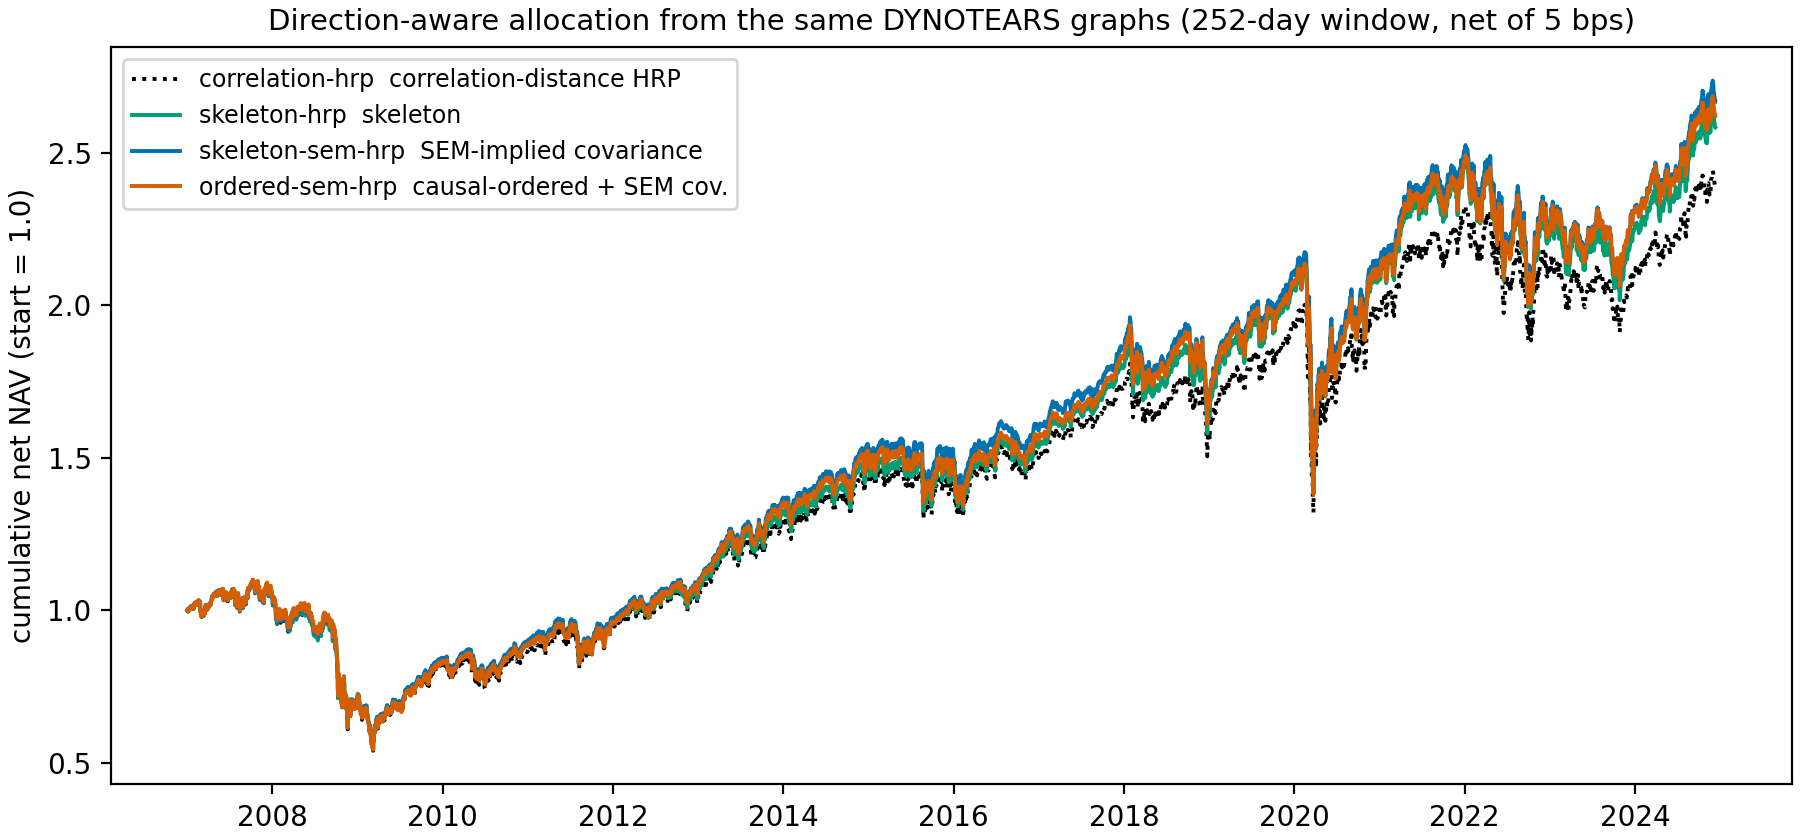
\includegraphics[width=0.99\textwidth]{figures/phase_ii_nav.png}
  \caption{Cumulative net NAV, one-year window: the correlation control
    \HRP{}, the skeleton \skelsamp{}, and the orientation-aware \skelsem{}
    and \orientsem{}. All variants absorb the full ${\approx}50\%$ GFC
    drawdown; the study concerns relative allocation quality, not
    drawdown avoidance.}
  \label{fig:nav}
\end{figure}

\subsection{Robustness to design parameters}

\paragraph{Sparsity ($\tau$).} Thresholding the graph at
$\tau\in\{0,0.01,0.05,0.10\}$ leaves the treatment flat-to-better
(\orientsamp{}:
$0.399\to0.402$ at the heaviest threshold) while the
skeleton control drifts down ($0.403\to0.394$; Table~\ref{tab:tau}), so
the orientation-aware
allocators are not artefacts of the regularisation threshold. These sweep
differences are point estimates; they were not formally tested.

\paragraph{Costs and turnover.} The covariance-channel increment is
cost-invariant in point estimates: \skelsem{}$-$\skelsamp{} at two years
moves from $+0.022$ to $+0.025$ as
costs rise from 0 to 20\,bps (differences on unrounded series;
Table~\ref{tab:cost}), because \skelsem{}'s turnover ($0.102$
one-way per
rebalance) is below the control's ($0.112$). The claim does not extend
to the ordering route at short windows: \orientsem{} carries the
family's highest turnover ($0.140$), and its one-year increment erodes
from $+0.004$ at zero cost to $0.000$ at 20\,bps, while its two-year
increment survives the sweep. The covariance channel does not win by
trading less and is not eroded by trading more; the ordering channel at
one year is.

\paragraph{Discovery method.} Under VARLiNGAM graphs the orientation effect
is absent at all four windows (4 of 12 contrasts positive, mean $-0.005$;
Figure~\ref{fig:forest}, right, and the grey series of
Figure~\ref{fig:gradient}). The decomposition is therefore
method-dependent: DYNOTEARS' jointly-optimised, acyclicity-constrained
$W$ supports orientation-aware allocation where VARLiNGAM's ICA-ordered
$B_0$ does not. This is consistent with VARLiNGAM's identification
weakening as
residuals Gaussianise over longer windows and, at the nine-month window,
with its unpruned $B_0$ saturating in the thin-sample regime (density
$32\%$ against DYNOTEARS' stable $6$--$7\%$;
Section~\ref{sec:asset-graph}),
so its short-window graphs carry little usable orientation signal either.
A DYNOTEARS graph supplies two things at once, the direction of each
edge and a fitted magnitude for it, so its cells alone cannot show which
of the two the orientation effect consumes; the ridge-Granger control
separates them, preserving a usable ordering while degrading the
magnitudes. It thereby localises where inside
the orientation the value sits: causal-ordered bisection survives on its
graphs (\orientsamp{} $=0.393$ vs DYNOTEARS' $0.399$) while the
SEM-covariance
allocator collapses (\skelsem{} $=0.352$; gap $-0.060$,
$p=0.11$). A ridge-VAR coefficient matrix carries a serviceable
ordering but not structural effect sizes, so the dissociation indicates
that orientation's contribution does not lie in merely knowing which way
the
arrows point (an ordering survives even a one-lag ridge regression)
but in edge magnitudes trustworthy enough to propagate shocks, the
ingredient only the jointly-optimised DYNOTEARS fit supplies. This is a
refinement of the answer to the research question, not a separate benchmark: ``orientation''
pays through its weighted, propagatable form.

\paragraph{A second family member (HERC).} Chapter~\ref{chap:background}'s
family-wide framing is an interface claim: any hierarchical allocator
clustering on a symmetric matrix discards orientation, whatever its
tree-reading rule. Whether the measured decomposition
generalises across tree-reading rules is a separate, empirical
question, tested on a second member with interpretations committed
before any cell was run (\texttt{PREDICTIONS\_HERC.md}): a
full-recursion Hierarchical Equal Risk Contribution allocator
\cite{raffinot2018herc}, identical to the HRP family in clustering
stage and cluster-risk measure but descending the dendrogram's actual
topology instead of bisecting the leaf ordering. The outcome is mixed
and bounds the generalisation: the orientation channel's sign carries
at every window, the skeleton channel's does not, and the whole HERC
family sits well below its HRP counterparts (cells and contrasts in
Appendix~\ref{app:tables}). The decomposition's magnitudes are
therefore allocator-specific: what generalises to this second member
is orientation's sign, and the family-wide claim is retained only in
its interface form. All twelve HERC cells join the deflation universe
and neither SPA family.

\subsection{Regime dependence}
\label{sec:regimes}

The prior-verification result (Section~\ref{sec:discovery-run}) showed
edge assignment matters most in stress windows, motivating the
hypothesis that orientation-aware allocation would add most value in
crises. The regime-conditional analysis contradicts this: at the
one-year window the orientation-aware allocators' edge over the \HRP{}
control concentrates in the bottom VIX quintile ($+0.29$/$+0.31$
Sharpe for \skelsem{}/\orientsem{}) and is slightly negative in the
top quintile, while in NBER recessions the skeleton allocator is the
strongest (Figure~\ref{fig:regime} and Table~\ref{tab:regime-full},
Appendix~\ref{app:tables}). These figures are descriptive: no formal
regime-level test was run, and conditional Sharpe levels are
mechanically inflated in the calm regime, so only within-regime
differences are read. A plausible reading is that in stress,
correlations rise toward one and any structure is swamped by the
common factor, while in calm markets cross-sectional causal
heterogeneity is the signal. Whatever the mechanism, the hypothesis as
stated was wrong and is reported as such, an outcome that Howard et
al.'s stable-regime centrality alpha (Section~\ref{sec:howard-theme})
had anticipated.

\section{Multiplicity-aware adjudication}
\label{sec:believe-rigour}

% Numbers in this section come from _generated/robust_stats.tex, regenerated
% by `python -m scripts.robust_stats --phase-ii` over all evaluated bundles.

\paragraph{Non-normality and selection bias (PSR/DSR).} Every headline
allocator's Probabilistic Sharpe ratio (the probability its true Sharpe
exceeds zero given the sample's higher moments) is high (\HRP{}
$\rsCorrPSR$, \skelsamp{} $\rsVprimePSR$, \skelsem{} $\rsDonePSR$ at
one year), so the
levels are not fat-tail artefacts. Deflating against the best Sharpe
expected from \rsNtrials\ no-skill trials, the study's highest Deflated
Sharpe ratio belongs to \orientsem{} at the 18-month window
($\rsDtwosDSRWthree$), followed by the direction-free de-factored
control ($\rsDdfDSRWthree$) and \skelsem{} ($\rsDoneDSRWthree$), against
the control's $\rsCorrDSR$ and the skeleton's
$\rsVprimeDSR$; the top of the deflation table is filled by the
orientation-aware cells and the de-factored control that mimics them,
itself consistent with the mechanism finding of
Section~\ref{sec:orientation-role}. The ordering of the decomposition survives deflation;
how much of its statistical separation survives is what the family-wise
tests size next.

\paragraph{Family-wise comparisons (SPA).} Two SPA families
adjudicate the claims with the search priced in, and every window-level
test is run twice: first over the full allocator grid (all
seven graph-consuming allocators of the experiment plan, both discovery
methods), then over the
narrower family the report's taxonomy defines (the $2\times2$ crossing
plus the second symmetrisation control). The narrowing was fixed only
after the four-window results had been seen, so the full grid's
numbers are the primary ones and the narrowed family's are reported
second and labelled as such. The two families, (i)
the causal family vs the \HRP{} control and (ii) the
orientation-aware variants vs the shared skeleton control (\skelsamp{}
on DYNOTEARS graphs; Section~\ref{sec:decomposition}), are tabulated in
Table~\ref{tab:spa}, whose final column prices the search across
strategies and the four estimation windows in a single pooled
family against the one-year control.

\begin{table}[t]
  \centering
  \caption{Hansen's SPA consistent $p$-values by family, window and
    grid. ``Pooled'' runs one SPA whose candidate set is the union of
    the family's cells at all four windows against the family's one-year
    control, so it prices the strategy search and the window search
    jointly. Bold: $p<0.05$.}
  \label{tab:spa}
  \small
  \begin{tabular}{l l c c c c c}
    \toprule
    Family & Grid & 189 & 252 & 378 & 504 & Pooled \\
    \midrule
    (i) vs \HRP{}      & full     & $\rsSpaSkelWonePre$ & $\rsSpaSkelWtwoPre$ & $\rsSpaSkelWthreePre$ & $\rsSpaSkelWfivePre$ & $\rsSpaSkelPooledPre$ \\
    (i) vs \HRP{}      & narrowed & $\rsSpaSkelWone$ & $\rsSpaSkelWtwo$ & $\mathbf{\rsSpaSkelWthree}$ & $\mathbf{\rsSpaSkelWfive}$ & $\rsSpaSkelPooled$ \\
    (ii) vs \skelsamp{} & full     & $\rsSpaDirWonePre$ & $\rsSpaDirWtwoPre$ & $\rsSpaDirWthreePre$ & $\rsSpaDirWfivePre$ & $\rsSpaDirPooledPre$ \\
    (ii) vs \skelsamp{} & narrowed & $\rsSpaDirWone$ & $\rsSpaDirWtwo$ & $\rsSpaDirWthree$ & $\mathbf{\rsSpaDirWfive}$ & $\rsSpaDirPooled$ \\
    \bottomrule
  \end{tabular}
\end{table}

In sum: under the full grid nothing rejects. Every
window-level rejection quoted in this report
($p=\rsSpaSkelWthree$--$\rsSpaDirWfive$, the longest estimation windows of
families (i) and (ii)) exists only under the post-hoc narrowing.
The pooled column completes the multiplicity accounting on the axis the
per-window tests leave unpriced, and it is decisive in the deflationary
direction: once the window search is priced alongside the strategy
search, nothing rejects for either family, under either grid
($p=\rsSpaSkelPooled$ for the narrowed causal family,
$\rsSpaDirPooled$ for the narrowed orientation family). The
window-level rejections are therefore read as
suggestive rather than established: they coincide with the peaks of
the point estimates, but survive neither the full grid nor the joint
pricing of the window search.

\paragraph{The Model Confidence Set.} The $90\%$ MCS over the
distinct one-year strategies retains every member of the reported
family and both graph-blind controls. This is best read as a statement
about
power, not a vindication of everything retained: with this many highly
correlated long-only variants whose Sharpes span $0.35$--$0.41$, the
equivalence test lacks the power to rank the causal family, including
separating treatments from controls.

\paragraph{Verdict on the research question, with uncertainty stated.} The decomposition's
point estimates are clear and internally consistent: a stable total
gain whose composition shifts with the estimation window (skeleton hump-shaped and
peaking at the one-year convention, orientation positive at every window
and largest at the extremes), with the orientation-aware allocators
topping the study-wide DSR table. Its statistical support is
modest and reported at its estimated size: 36 of 40
graph-versus-correlation cells
positive; one pairwise-significant orientation cell among twelve
($p=0.048$); no family-wise rejection
anywhere under the full grid; marginal rejections at the longest
estimation windows under the post-hoc narrowed family only, coinciding
with the peaks of the point estimates; and no rejection for either
family once the pooled test
prices the window search alongside the strategy search
(Table~\ref{tab:spa}). The mechanism controls of
Section~\ref{sec:orientation-role} land asymmetrically. The
orientation channel's covariance gain is
reproduced by a graph-free de-factored covariance, so it is
robustness, not directional information as such; the skeleton
channel's one-year gain is not reproduced by a graph-free skeleton of
matched density, so the paying region at the conventional window does
need the discovered graph. The
largest defensible claim is modest: replacing the correlation
matrix with a DYNOTEARS graph pays through the skeleton near the
one-year convention, and keeping the orientations costs nothing while
improving robustness to the estimation-window choice. The evidence
does not support attributing the covariance-channel gain to edge
direction, any orientation effect under VARLiNGAM graphs, or the
stress hypothesis. That profile, precise sign-consistent point
estimates whose family-wise support appears only under the post-hoc
narrowing, and whose leading mechanism a direction-free control
reproduces, is the finding.

\section{An out-of-sample slice}
\label{sec:oos}

Every result so far shares the 2007--2024 panel, and
Section~\ref{sec:believe} discloses three design choices that were
informed by results on that panel. A deflation correction is not a
substitute for out-of-sample replication, so I ran one: the identical
harness, universe, cost model and DYNOTEARS configuration on
2025-01 to 2026-07, a span that did not exist when the design was
fixed. The protocol and the interpretation of every possible outcome
were committed before any out-of-sample price was fetched
(\texttt{PREDICTIONS\_OOS.md}), including this constraint, stated in
advance: 19 monthly rebalances (399 trading days) put the standard
error of an annualised Sharpe near $0.8$ and of the pairwise contrasts
near $0.08$, so the slice is a sign and magnitude check on the
point estimates, and no $p$-value computed on it counts as evidence in
either direction. Two protocol notes: CRSP daily data ends 2024-12-31,
so the slice's prices come from Yahoo Finance (the source switch is
confined to the slice and disclosed here), and all 99 names remained
listed throughout it.

\begin{table}[t]
  \centering
  \caption{Out-of-sample contrasts (net $\Delta$Sharpe,
    2025-01 to 2026-07, point estimates only). Every sign the
    protocol specified in advance is consistent with the in-sample
    decomposition;
    at this sample length the contrast standard errors are roughly
    $0.08$, so magnitudes are not interpreted.}
  \label{tab:oos}
  \small
  \begin{tabular}{l c c c c}
    \toprule
    & \multicolumn{4}{c}{Window (days)} \\
    \cmidrule(lr){2-5}
    Contrast & 189 & 252 & 378 & 504 \\
    \midrule
    skeleton: \skelsamp{} $-$ \HRP{}          & $\rsOosSkelWone$ & $\rsOosSkelWtwo$ & $\rsOosSkelWthree$ & $\rsOosSkelWfive$ \\
    orientation: \skelsem{} $-$ \skelsamp{}   & $\rsOosOrientWone$ & $\rsOosOrientWtwo$ & $\rsOosOrientWthree$ & $\rsOosOrientWfive$ \\
    orientation: \orientsem{} $-$ \skelsamp{} & $\rsOosOrientBothWone$ & $\rsOosOrientBothWtwo$ & $\rsOosOrientBothWthree$ & $\rsOosOrientBothWfive$ \\
    total: \skelsem{} $-$ \HRP{}              & $\rsOosTotalWone$ & $\rsOosTotalWtwo$ & $\rsOosTotalWthree$ & $\rsOosTotalWfive$ \\
    residual: \skelsem{} $-$ de-factored      & $\rsOosResidWone$ & $\rsOosResidWtwo$ & $\rsOosResidWthree$ & $\rsOosResidWfive$ \\
    \bottomrule
  \end{tabular}
\end{table}

The outcome matches the consistency reading
(Table~\ref{tab:oos}). The total gain is positive at all four windows,
the \skelsem{} orientation increment is positive at all four, and
\orientsem{}'s is positive from one year out with its only negative
cell at nine months, the window whose in-sample contributions already
carried the anchor-dependence caveat. The skeleton contribution,
hump-shaped in sample, is positive at every window here. The mechanism
reading also carries at point-estimate level: the graph-free
de-factored control again sits within $0.011$ of \skelsem{} at three
windows (and $0.020$ below it at two years), so out of sample too the
covariance channel behaves like de-factoring. One honesty note bounds
this: the slice is a strong bull market (control Sharpe levels of
$0.78$--$0.92$), so the absolute magnitudes are inflated relative to
the 2007--2024 panel and are not compared to it. Within the limits
committed in advance, every specified sign
came back consistent with the in-sample decomposition, on data that did
not exist when the design, the family and the question were fixed.

\section{Threats to validity}
\label{sec:believe}

\paragraph{Effect sizes sit near the detection floor.} The decomposition's
components are $0.01$--$0.03$ Sharpe over 18 years, against a full-sample
Sharpe standard error of ${\approx}\,\rsSharpeSEFull$ (Lo's
approximation on the $\sim$4{,}500-day sample). The pairwise contrasts
are far more precise, because the strategies are highly
correlated and the bootstrap differences the joint panel: the
block-bootstrap standard error of the total contrast
(\skelsem{}$-$\HRP{} at one year) is $\rsContrastSETotal$ and of the
orientation contrast (\orientsem{}$-$\skelsamp{}) $\rsContrastSEOrient$.
Those standard errors put numbers on ``underpowered'': at $5\%$ size and
$80\%$ power the one-sided minimum detectable effects are
${\approx}\,\rsContrastMDETotal$ and ${\approx}\,\rsContrastMDEOrient$
net Sharpe respectively, roughly twice the observed $+0.031$ total and
$+0.023$ orientation increments. The design could therefore only have
certified effects about double the size actually observed, and that cuts
both ways: the
rejections that do occur are marginal and narrowed-family only, and the
absence of rejection at
the shorter estimation windows is not evidence of absence. At the pairwise level, one
$p=0.048$ cell among twelve orientation contrasts is close to what
multiplicity predicts under the null, which is why no single cell is
claimed as a discovery; the orientation effect earns its standing from
the sign-consistency of the contribution across windows and treatments
(Section~\ref{sec:decomposition}), not from any single cell.

\paragraph{Forking-paths risk.} Three design choices were informed by
earlier results, and this section is their record. The choice of question
was informed by the results of the project's first phase, which took
Hierarchical Sensitivity Parity \cite{rodriguez2023hsp}
(Section~\ref{sec:hrp-theme}) as its starting point and replaced the
method's correlation-based driver selection with selection from the
discovered graph. That phase contributes \rsNtrialsPhaseI\ of the
\rsNtrials\ configurations in the deflation universe, including the two
skeleton cells that the replication gate of
Section~\ref{sec:ablation-design} targets; the graph route of this study
contributes the remaining \rsNtrialsPhaseII. Its two null results are
recorded in Appendix~\ref{app:hsp}. The window grid reached its
four-window form in two stages: the conventional 252- and 504-day windows
were evaluated first, and the 189- and 378-day windows were added when the
initial results suggested a composition shift that a two-point design
cannot distinguish from noise. Three disciplines bound the associated
risk: the added windows were run symmetrically (every allocator, both
methods, all cells reported); the deflation universe covers all
\rsNtrials\ configurations ever evaluated, both phases, all windows; and
the headline reading (orientation positive everywhere, largest at the
extremes) would have been weakened, and reported as such, had the added
windows come back inconsistent. The narrowed-family rejections inherit
the risk asymmetrically: the strongest (Premise 1 at 378 days,
$p=\rsSpaSkelWthree$)
sits on an added window, while the two-year rejections
($p=\rsSpaSkelWfive$, $\rsSpaDirWfive$) sit on windows evaluated from the
start, which bounds the concern for them.

The third informed choice is the family itself, and it is the most
consequential. The plan's grid contained seven allocators; the
narrowing to the five
allocators of the two-entry-point taxonomy of
Chapter~\ref{chap:sensitivity} was made after the four-window results
had been seen. The taxonomy is a principled reason for the smaller
family (the thesis question is about HRP's two entry points, and those
two arms enter the graph elsewhere: both are further
orientation-consuming allocators, one replacing the hierarchy with risk
parity over structural shocks, the other building the clustering
distance from shared upstream ancestry), but the timing means the narrowed
family's rejections cannot be read as
confirmatory, and it is exactly the choice
the significance turns on: every family-wise number is therefore
reported for both families in Table~\ref{tab:spa}, where the full grid
rejects nowhere on the window axis and the narrowed family supplies
every rejection. The two excluded arms stay in the deflation universe,
and their results are directionally consistent with the family they were
excluded from (above the control in all sixteen of their cells, both
discovery methods and all four windows, by $+0.002$ to $+0.024$), so
the exclusion is not results-driven in
direction, but the reader should weigh the narrowed-family rejections
with the timing in view. Separately, the two mechanism controls of
Section~\ref{sec:orientation-role} were added after this chapter's
results were first drafted, in response to the objection that
$\Sigma_{\mathrm{SEM}}$'s gain might be generic; their interpretations
were written down and committed before either control was run, and they
join the deflation universe but neither family.

\paragraph{Single asset class, one universe, approximated index.} Everything
here concerns long-only allocation within ${\sim}100$ US large-caps; every
variant absorbs the full ${\approx}50\%$ GFC drawdown. Whether the
decomposition transfers to universes with richer exogenous structure
(multi-asset, credit, commodities) is untested. The top-by-market-cap
approximation of the S\&P~100, the fixed snapshot-union universe (whose
membership is partly settled by market caps realised later in the
sample) and the absence of delisting returns
(Section~\ref{sec:asset-graph}) carry
mild residual survivorship and look-ahead effects. Their sign is
favourable, but they are shared by every allocator on the same panel, so
they inflate the absolute levels rather than the pairwise contrasts the
thesis is about; quantifying them with a point-in-time universe is left
to future work.

\paragraph{Method-dependence is a caveat on the mechanism.} The orientation
effect exists under DYNOTEARS graphs only. Until a second discovery method
reproduces it, the safest interpretation is ``DYNOTEARS' contemporaneous
structure supports orientation-aware allocation'', not ``causal orientation
in markets is allocatively valuable''. The verdict of
Section~\ref{sec:believe-rigour} stands as this chapter's summary.
% ===== chapters/06_conclusion.tex =====
% ============================================================
\chapter{Conclusions and Future Work}
\label{chap:conclusion}
% ============================================================

\section{Summary of findings}
\label{sec:summary}

This thesis asked one question: when the correlation matrix in
hierarchical portfolio allocation is replaced by a causal graph, is
there a performance improvement, and how much of any improvement is
attributable to the graph's skeleton
versus its edge orientations? It made the question answerable by building
the
machinery it presupposes: a reproducible rolling discovery pipeline that
delivers the identical asset--asset DAG to every allocator
(Chapter~\ref{chap:discovery}), and an orientation-aware allocator family
with skeleton and correlation controls verified orientation-blind under
stated invariances (Chapter~\ref{chap:sensitivity}), which discharges
Premise 2. It then answered the question under multiplicity-,
distribution- and stability-aware inference (Chapter~\ref{chap:evaluation}).

The answer, in summary: the causal graph's gain over the
correlation matrix is stable across estimation windows, but its source
shifts: against the primary skeleton control, the skeleton pays most
clearly near the conventional one-year window, while orientation pays at
every estimation window and, robustly to the choice of orientation-blind control,
from one year out. The between-window differences are about one standard
error, and the window grid was widened partway through, so the shapes
carry that uncertainty. Orientation buys robustness to the estimation
window, not level, and a direction-free de-factored covariance
reproduces that robustness, so its mechanism is market-factor removal
rather than directional content. Family-wise, nothing rejects over the
full allocator grid of every strategy the experiment plan evaluated;
support reaches conventional significance
only under the narrower reported family, at the longest estimation windows,
marginally, where the point estimates also peak. In detail (net annualised Sharpe, 2007--2024,
monthly
rebalancing, 5\,bps costs, windows of 189/252/378/504 trading days):

\begin{enumerate}[itemsep=2pt]
  \item The total gain is stable across estimation windows.
        Replacing the correlation matrix with the DYNOTEARS graph is
        worth $+0.018$ to $+0.032$ net Sharpe (\skelsem{} $-$ \HRP{})
        at every window, and 36 of 40 graph-versus-control cells are
        positive.
  \item Its composition shifts with the window. The skeleton's
        contribution is hump-shaped and peaks at the one-year
        convention; orientation's is positive everywhere and U-shaped,
        largest where the sample moments are weakest. Orientation buys
        robustness to the estimation window, not level, and at the
        18-month window \orientsem{} attains the highest Deflated
        Sharpe ratio of all \rsNtrials\ configurations evaluated
        ($\rsDtwosDSRWthree$).
  \item The mechanism needs no graph; the skeleton does. A
        de-factored covariance with no graph reproduces the
        covariance-channel gain at every window, so the orientation
        robustness works through market-factor removal; the matching
        graph-free skeleton control fails to reproduce the skeleton's
        one-year gain, so the channel that pays at the conventional
        window does need the discovered graph
        (Section~\ref{sec:orientation-role}). The shapes themselves
        are anchor-dependent at nine months (limitation (vii)).
  \item Family-wise support depends on the family, and the
        full grid does not reject. Every SPA test runs over both the
        full seven-allocator grid and the narrowed five-allocator
        family fixed after the results were seen: the full grid rejects
        nowhere, the narrowed family rejects marginally at the longest
        estimation windows only, and the pooled test that prices the
        strategy and window searches jointly rejects for neither family
        (Table~\ref{tab:spa}). The $90\%$ Model Confidence Set declines
        to separate treatments from controls.
  \item The effect is method- and allocator-specific. Under
        VARLiNGAM graphs orientation adds nothing at any window
        (limitation (ii)); under the magnitude-degraded ridge-Granger
        control the ordering survives but the SEM covariance collapses,
        so the value sits in trustworthy edge magnitudes; and on a
        second family member (HERC) only orientation's sign generalises
        (Section~\ref{sec:decomposition}). Descriptively, the edge
        concentrates in calm regimes; the stress hypothesis is
        rejected.
\end{enumerate}

\section{Contributions}
\label{sec:contributions}

The contribution of this thesis is the orientation-aware allocator family
and the fixed-graph ablation design; the decomposition of
Chapter~\ref{chap:evaluation} is what that instrument found. That single
claim unpacks into a methodological core and two strands that flow from
it:

\begin{itemize}[itemsep=2pt]
  \item Methodological (the core): the orientation-aware allocator family
        (SEM-implied, de-standardised, residual-calibrated
        covariance allocation, and causal-ordered bisection, which replaces
        the clustering dendrogram with the DAG's topological order),
        together
        with the fixed-graph ablation design that makes skeleton and
        orientation separately measurable, with controls verified
        orientation-blind under stated invariances. To my knowledge, both the family and the decomposition are
        new; the closest prior work \cite{howard2025causal} never sets
        weights from its graphs.
  \item Empirical (what the instrument found): the decomposition itself, traced across four
        estimation windows (a stable total; skeleton hump-shaped and
        peaking at the one-year convention against the primary anchor;
        orientation positive at every
        estimation window against that anchor and robustly so from one year out;
        family-wise support absent under the full grid and
        marginal, confined to the longest estimation windows, under the narrowed
        family), the identification of its covariance-channel mechanism
        as market-factor removal by a direct control, and its
        method- and
        regime-dependence.
  \item Meta-scientific: a
        reproducible, fully deterministic pipeline (including a
        data-determinism defect
        whose fix overturned two previously-drawn conclusions), with
        every design extension disclosed as such, all cells
        cache-verified, and the
        harness gated on an exact replication of the prior phase's
        result.
\end{itemize}

\section{Limitations}
\label{sec:limitations}

(i) The decomposition's components are
$0.01$--$0.03$ Sharpe: near the 18-year detection floor, individually
non-significant against the stronger controls, and quantifiably
underpowered: the one-sided minimum detectable effects at $80\%$ power
are ${\approx}\,\rsContrastMDETotal$ (total) and
${\approx}\,\rsContrastMDEOrient$ (orientation) net Sharpe, roughly
twice the observed increments (Section~\ref{sec:believe}).
The point estimates are exactly reproducible; the inference, where it
clears the family-wise bar, is marginal, clears it only under the
post-hoc narrowed family, not under the full grid, and does not survive
pricing the window search jointly with the strategy search.
(ii) The
orientation effect exists under one discovery method (DYNOTEARS); until
another method reproduces it, it should be read as a property of DYNOTEARS'
contemporaneous structure, not of markets, and the de-factored control
shows its covariance channel is reproducible with no graph at all
(the skeleton channel's one-year gain, by the matching control, is
not). (iii) Long-only US
large-cap equity only; every variant absorbs the full ${\approx}50\%$ GFC
drawdown; transfer to richer universes is untested. (iv) The
universe approximates the S\&P~100 by market-cap ranking and a fixed
snapshot union, with mild residual survivorship effects. (v) The
asset-block SEM marginalises over the macro drivers, so the structural
shocks' assumed independence is an approximation. (vi) The choice
of research question was informed by the results of the first phase
(the Hierarchical Sensitivity Parity route, \rsNtrialsPhaseI\ of the
\rsNtrials\ trials), the window grid was widened to four estimation windows partway through
the study, and the family-wise comparison set was narrowed from the
full seven-allocator grid to five after the results were seen
(Section~\ref{sec:believe}); all three are disclosed, both families'
numbers are reported, and the unified
\rsNtrials-trial deflation universe prices in every configuration the
search ever touched, but a deflation correction is not a substitute for
out-of-sample replication. The 2025--26 slice
(Section~\ref{sec:oos}), whose protocol was fixed before the data
existed, supplies the directional part of that
replication: every sign it specified came back
consistent; at 19 months
it can certify signs and nothing more, so the significance question
stays open. (vii) At the shortest window the two
orientation-blind controls themselves disagree (\skelalt{} $-$ \skelsamp{} $= +0.025$,
$p=0.013$), so the nine-month contributions carry extra estimator
uncertainty;
more generally the hump and U shapes of the decomposition are anchored on
\skelsamp{}, and under the \skelalt{} anchor the skeleton contribution is
flat
and the nine-month orientation contribution slightly negative
(Section~\ref{sec:decomposition}). (viii) Month-to-month
persistence of the discovered edges was not quantified: graph stability
over time is attested by the determinism of the fits and the stability of
aggregate diagnostics, not by an edge-overlap measure.

\section{Broader impact}
\label{sec:impact}

\paragraph{For investors.} Allocation research is consumed by asset
managers
and pension schemes, so its failures are borne, diffusely and years
later, by end savers. The characteristic harm in this literature is not a
malfunctioning system but a convincing backtest of an overfit strategy;
multiplicity-corrected, family-wise-honest evaluation is therefore not
methodological decoration but the investor-protection function of research
method, and this report applies it to its own headline. The same honesty is
a corrective to what might be called causal-washing: a ``causal''
label invites over-trust, and the finding here is that a causal method's
value can be modest, window- and method-dependent, and, at the
conventional one-year window, largely attributable to structure that
cheap symmetrisation already captures. The label guarantees nothing; the
decomposition, not the branding, is what carries information.

\paragraph{For the field.} One of this project's technical choices
generalises into a norm. The determinism episode of Section~\ref{sec:cache}
(two conclusions
overturned by a reproducibility fix) argues that reproducibility
belongs among publication prerequisites rather than aspirations; the
deterministic, seed-free construction of the allocator family is the
design corollary, and it is what makes every number in this report
exactly replicable.

\paragraph{Costs.} The content-keyed cache cut the marginal cost of a
configuration from ${\sim}15$ hours to ${\sim}40$ seconds, which is what
made an \rsNtrials-configuration study, and hence its multiplicity
correction, affordable at all. The compute and energy economics of
caching-first experimental design are a transferable, if unglamorous,
contribution to sustainable empirical research: rigour and efficiency were
complements here, not a trade-off.

\section{Future work}
\label{sec:future}

(1) A second orientation source. The decomposition's biggest caveat
is method-dependence: repeating the fixed-graph ablation on graphs from a
different family (e.g.\ the non-linear NTS-NOTEARS, whose prior-transfer was
verified in a reduced-scope probe but whose ${\sim}10\times$ fit cost
deferred a full backtest) would test whether orientation value is a
DYNOTEARS artefact. (2)
Signed structural allocation. Equalising risk contributions over
structural shock origins (where risk enters the causal system)
rather than over correlated returns is the natural next use of
$\Sigma_{\mathrm{SEM}}$; a long-only variant was among the seven
allocators of the pre-registered grid and is priced into the full-grid
tests of Section~\ref{sec:believe-rigour}, but exact per-shock parity
generally requires
shorting, so a long--short mandate, not the long-only setting studied here,
is its natural home. (3) Richer universes, where cross-asset
causal chains are plausibly longer-lived than among 99 co-moving
large-caps:
multi-asset-class portfolios are where the skeleton/orientation split
could materially differ. (4) Orientation-aware risk attribution.
The
total-effect matrix $B$ supports ex-post decompositions, attributing a
month's loss to the shocks that drove it, that the correlation toolkit
cannot express;
worthwhile even where the allocation gain is modest. The
infrastructure built here (the deterministic pipeline, the discovery cache
and the ablation harness) makes each of these a matter of days, not
months, of compute, which, as this project found twice, is a prerequisite
for trusting the answers.

% End matter
\clearpage
\printbibliography[heading=bibintoc, title={References}]

\chapter*{Declarations}

\section*{Use of Generative AI}
I acknowledge the use of Opus 4.6--5 and Fable 5 
(Anthropic, \url{https://claude.ai/}) as coding assistants
and as drafting and proofreading aids. 
I confirm that no content generated by AI has been presented as my own work.

\section*{Ethical Considerations}
There are no ethical issues associated with this project.

\section*{Sustainability}
All work was done on my laptop: no additional resources were used.

\section*{Availability of Data and Materials}
The source code and data are publicly available at
\url{https://github.com/j-muthu/portfolio-optimisation-causal-networks}.
The raw market data is licensed from WRDS/CRSP and cannot be distributed,
but the results can still be reproduced from the above repository.

\appendix
% ===== chapters/A_appendix.tex =====
% ============================================================
\chapter{Supplementary Tables and Reproducibility}
\label{app:tables}
% ============================================================

This appendix collects the full tables behind Chapter~\ref{chap:evaluation}
and the reproducibility notes. The report stands without it. One convention:
all $\Delta$Sharpe values quoted in the main text are computed on unrounded
return series; differencing the three-decimal entries below can therefore
disagree with a quoted increment by one unit in the third decimal.

\section{The full allocator matrix}

Table~\ref{tab:matrix-full} gives every cell of the fixed-graph ablation
(net annualised Sharpe) plus the supporting arms. The ridge-Granger control's
scope is deliberately narrow, covering one representative allocator per way
of
consuming the graph (skeleton \skelsamp{}, magnitudes \skelsem{}, ordering
\orientsamp{}) at the
one-year window, since its role is to dissociate ordering from
magnitudes, not to serve as a third full arm.

\begin{table}[h]
  \centering
  \caption{Net annualised Sharpe, 2007--2024, by graph source, allocator and
    window; row-wise best in bold. \HRP{} is graph-blind
    (method-independent). ``---'': outside the ridge-Granger control's
    representative-allocator scope.}
  \label{tab:matrix-full}
  \small
  \setlength{\tabcolsep}{4.5pt}
  \begin{tabular}{l l c c c c c}
    \toprule
    Graph & Window (days) & \skelsamp{} & \skelalt{} & \skelsem{} & \orientsamp{} & \orientsem{} \\
    \midrule
    DYNOTEARS & 189 & 0.387 & \textbf{0.411} & 0.408 & 0.392 & 0.408 \\
    DYNOTEARS & 252 & 0.403 & 0.398 & \textbf{0.411} & 0.399 & 0.406 \\
    DYNOTEARS & 378 & 0.402 & 0.409 & 0.415 & 0.405 & \textbf{0.419} \\
    DYNOTEARS & 504 & 0.372 & 0.383 & 0.395 & 0.382 & \textbf{0.399} \\
    VARLiNGAM & 189 & 0.393 & 0.388 & 0.364 & 0.387 & \textbf{0.394} \\
    VARLiNGAM & 252 & \textbf{0.397} & 0.396 & 0.385 & 0.388 & 0.386 \\
    VARLiNGAM & 378 & 0.399 & 0.392 & \textbf{0.407} & 0.398 & 0.399 \\
    VARLiNGAM & 504 & 0.377 & \textbf{0.390} & 0.383 & 0.372 & 0.375 \\
    ridge-Granger   & 252 & 0.389 & --- & 0.352 & \textbf{0.393} & --- \\
    \midrule
    \multicolumn{2}{l}{\HRP{} control (windows 189/252/378/504):} &
    \multicolumn{5}{l}{$\rsCorrSharpeWone$ / $\rsCorrSharpe$ /
      $\rsCorrSharpeWthree$ / $\rsCorrSharpeWfive$.} \\
    \bottomrule
  \end{tabular}
\end{table}

\paragraph{Mechanism controls.} The two direction-free covariance
controls of Section~\ref{sec:orientation-role} (\skelsamp{}'s clustering,
DYNOTEARS graphs, allocation covariance swapped): Ledoit--Wolf shrunk,
$\rsDlwSharpeWone/\rsDlwSharpe/\rsDlwSharpeWthree/\rsDlwSharpeWfive$
across the four windows; de-factored (single-factor residual),
$\rsDdfSharpeWone/\rsDdfSharpe/\rsDdfSharpeWthree/\rsDdfSharpeWfive$.
The graph-free skeleton control (partial-correlation skeleton,
density-matched, sample covariance):
$\rsDpcSharpeWone/\rsDpcSharpe/\rsDpcSharpeWthree/\rsDpcSharpeWfive$.
All three join the deflation universe; none belongs to either
family-wise
comparison set. Their pre-committed interpretations are in the
repository files \texttt{PREDICTIONS\_COVARIANCE\_CONTROLS.md} and
\texttt{PREDICTIONS\_SKELETON\_CONTROL.md}, each committed
before the corresponding control was run.

\paragraph{The HERC second family member.} The full-recursion HERC arm
of Section~\ref{sec:decomposition} (pre-committed in
\texttt{PREDICTIONS\_HERC.md}), net Sharpe across the four windows:
correlation-distance control $0.325/0.320/0.292/0.245$; skeleton member
(\skelsamp{}'s distance) $0.122/0.128/0.303/0.205$; orientation member
($\Sigma_{\mathrm{SEM}}$) $0.240/0.259/0.321/0.297$. The orientation
contrast (orientation member $-$ skeleton member) is positive at every
window: $+0.119$, $+0.131$, $+0.018$, $+0.092$ (unadjusted bootstrap
$p=0.03$, $0.03$, $0.81$, $0.21$); the skeleton contrast (skeleton
member $-$ control) is not: $-0.203$, $-0.193$, $+0.011$, $-0.040$
($p \geq 0.16$). A mechanical reading of the level shortfall is an
interface interaction: under the house single-linkage pattern the
dendrogram is deeply chained, and walking its topology compounds
roughly a hundred sequential budget splits, which HRP's balanced
bisection never does; Raffinot's cluster-cut variant, which prunes the
walk, is the natural next member to test. All twelve cells
join the deflation universe and neither SPA family.

\begin{figure}[tbp]
  \centering
  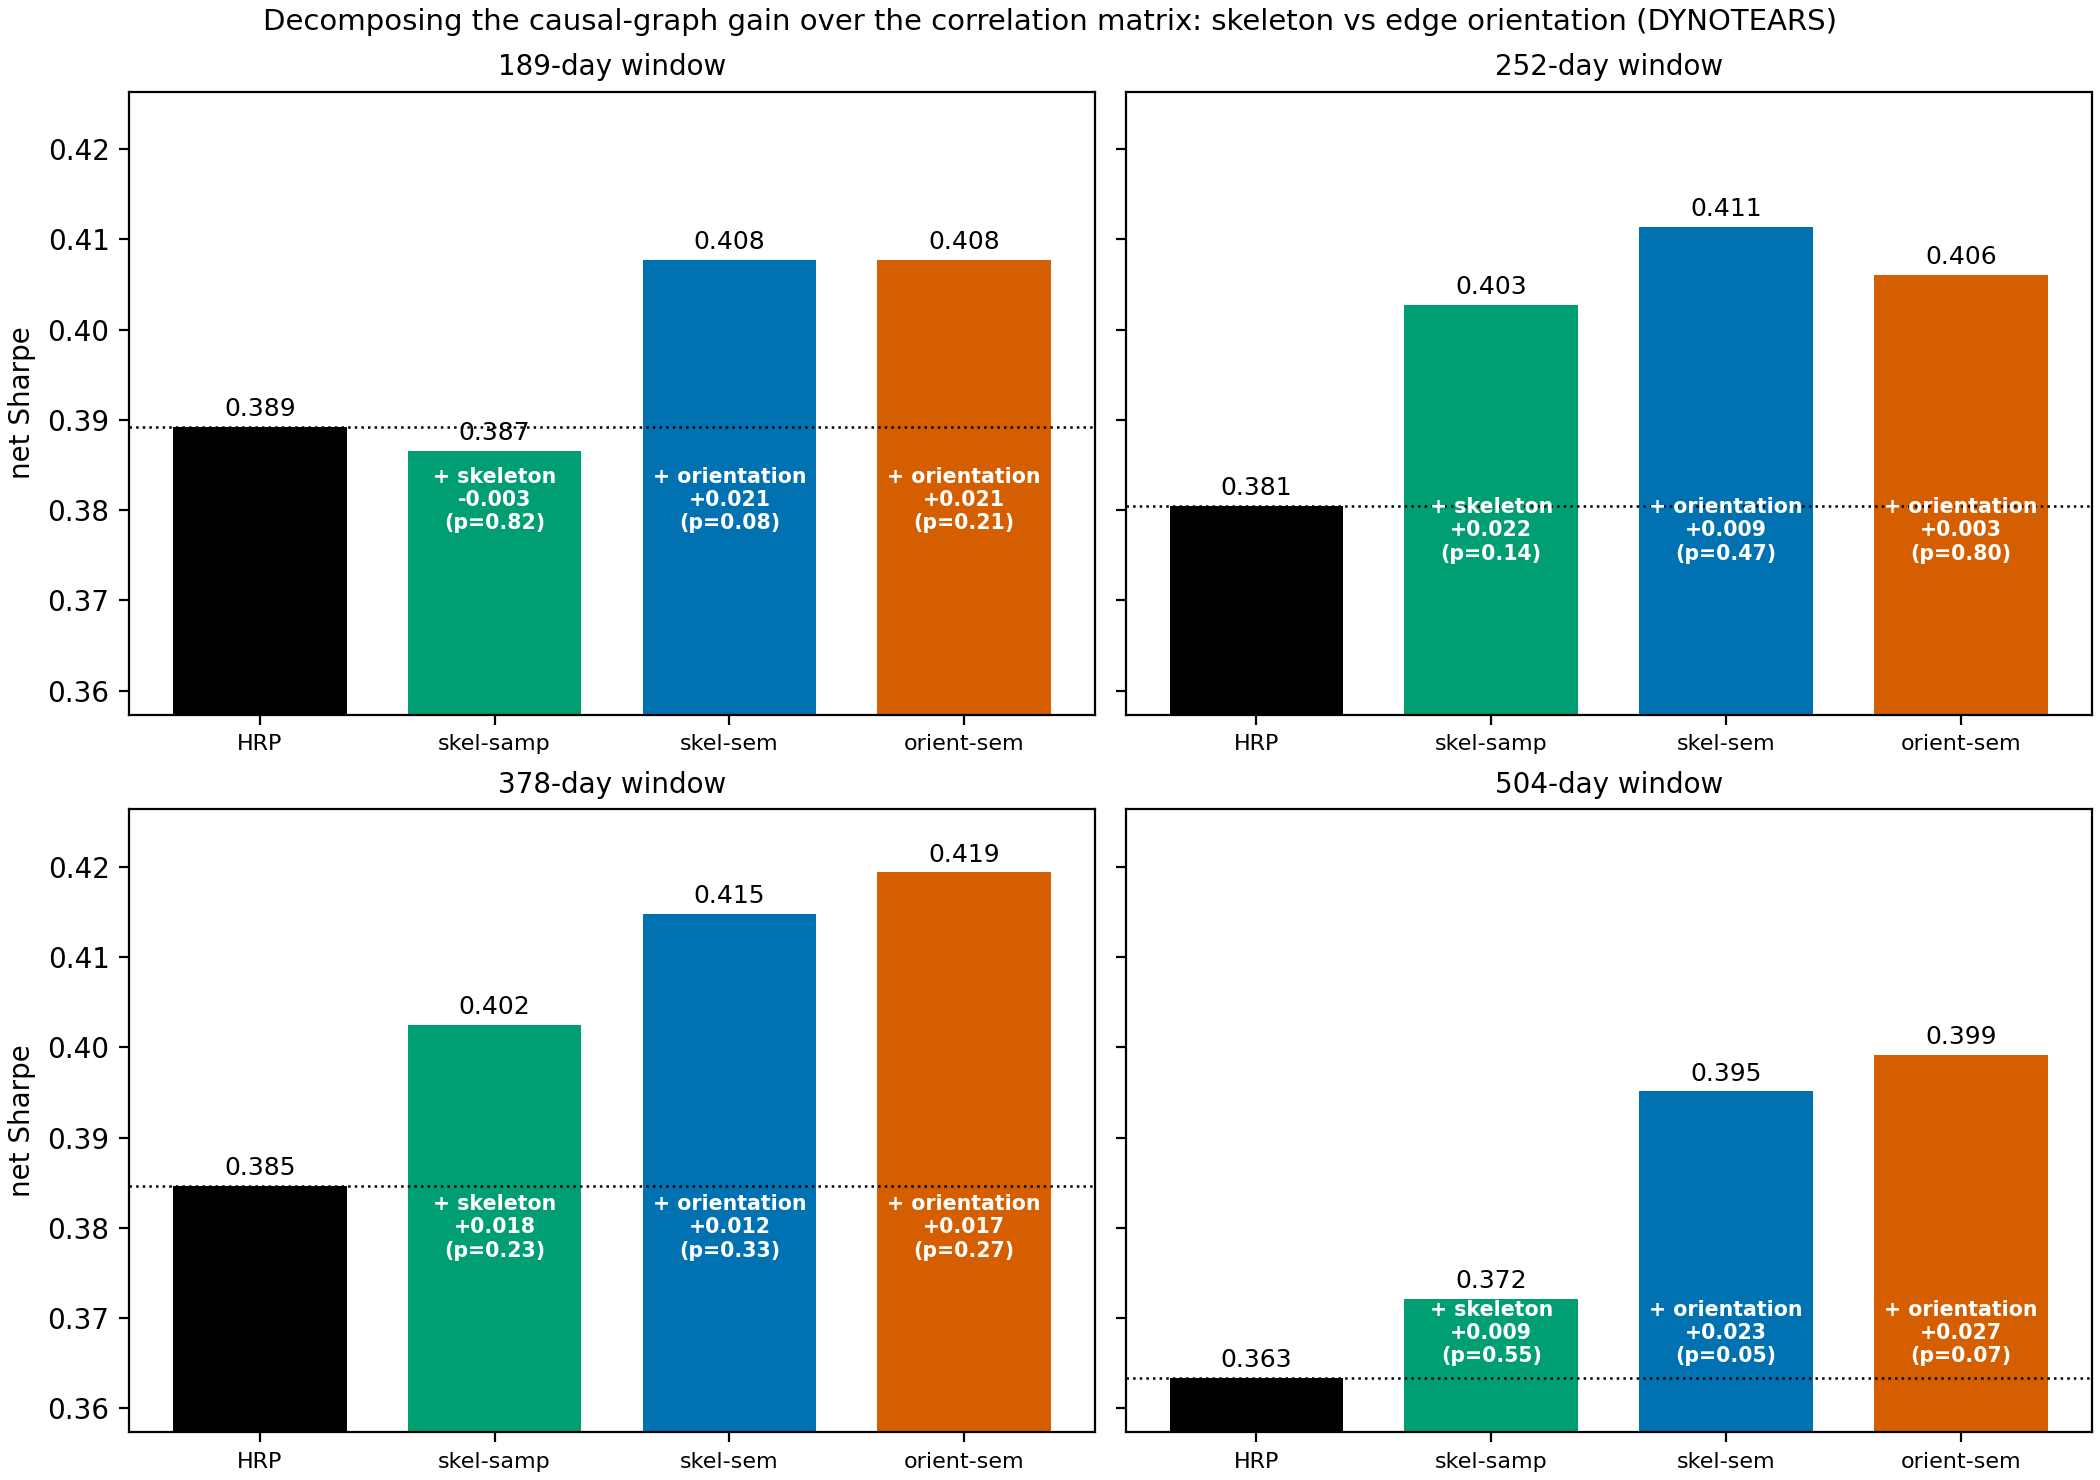
\includegraphics[width=0.99\textwidth]{figures/phase_ii_decomposition.png}
  \caption{The per-window levels behind Figure~\ref{fig:gradient}
    (DYNOTEARS graphs, net annualised Sharpe): \HRP{} $\to$ \skelsamp{}
    ($+$skeleton) $\to$ \skelsem{}/\orientsem{} ($+$orientation) at each estimation window,
    steps annotated with the pairwise bootstrap $\Delta$ and $p$-value.
    Section~\ref{sec:believe-rigour} adjudicates these steps family-wise.}
  \label{fig:decomp}
\end{figure}

\begin{figure}[tbp]
  \centering
  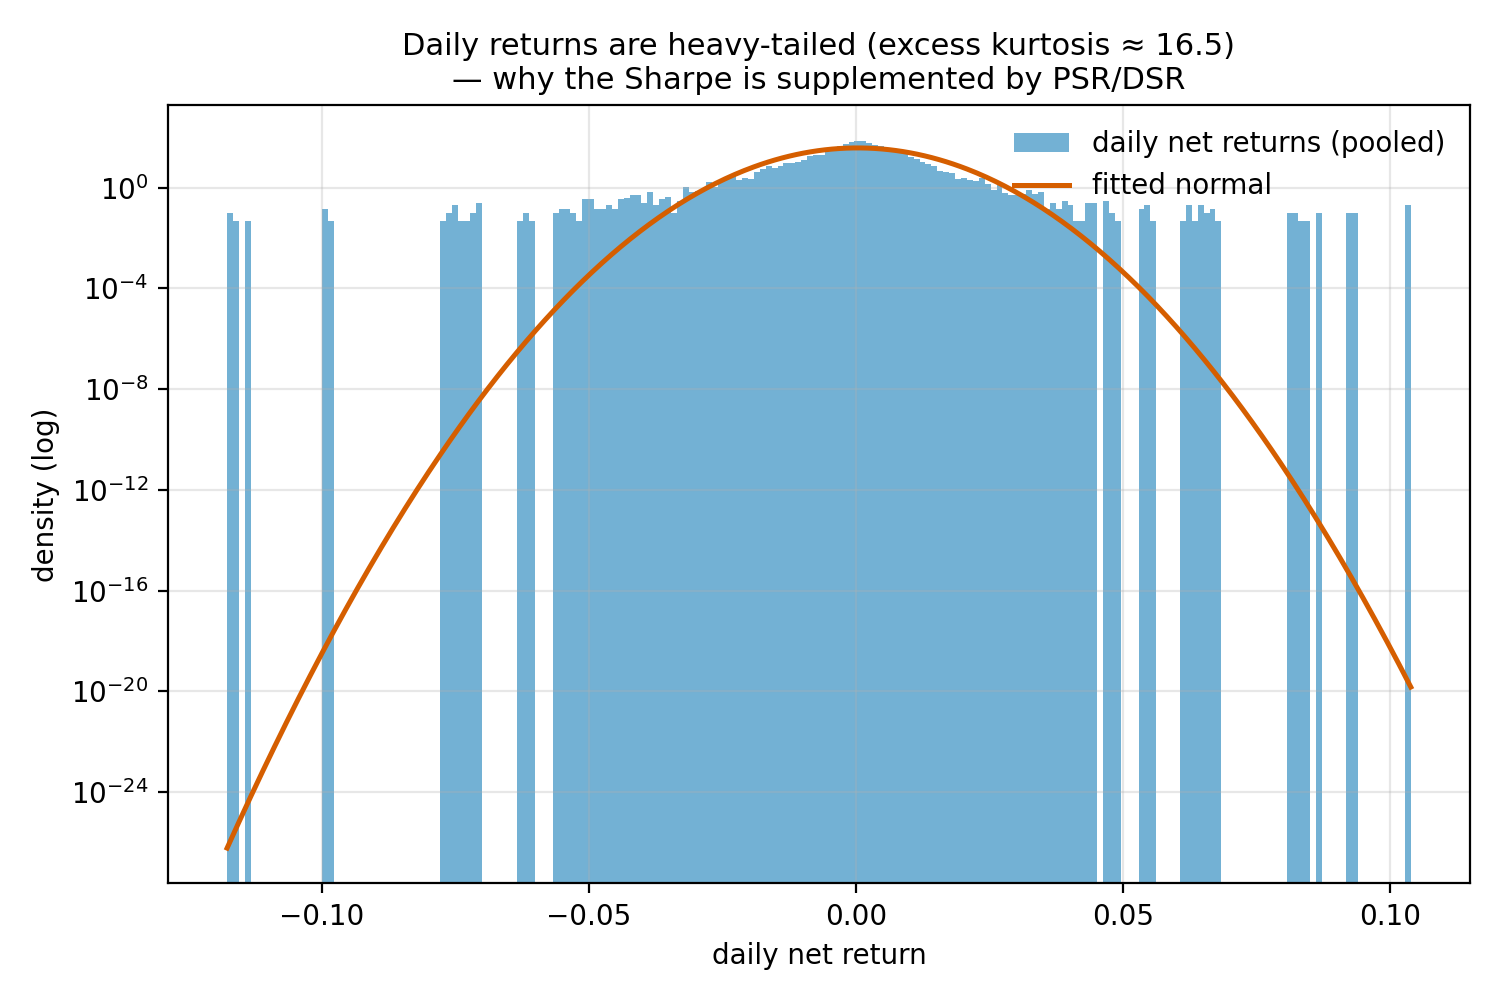
\includegraphics[width=0.7\textwidth]{figures/returns_distribution.png}
  \caption{Distribution of daily net returns (pooled across variants) against
    a fitted normal, log-density axis. The heavy tails (excess kurtosis
    ${\approx}\,\rsKurtosis$) are why the plain Sharpe ratio is supplemented
    by the Probabilistic and Deflated Sharpe ratios throughout.}
  \label{fig:retdist}
\end{figure}

\section{Headline configurations in return terms}

Table~\ref{tab:return-terms} restates the one-year headline cells in the
units an investor would recognise: net CAGR, maximum drawdown and
turnover. It is the source of the return-terms sentences of
Section~\ref{sec:r1}; the Sharpe column repeats
Table~\ref{tab:matrix-full} for orientation.

\begin{table}[h]
  \centering
  \caption{Net CAGR, maximum drawdown and mean one-way turnover per
    rebalance for the headline configurations at the one-year window
    (DYNOTEARS graphs; control from the shared harness). The naive
    anchors (equal weight, inverse variance) run on the identical
    calendar and cost model; equal weight's higher CAGR at lower Sharpe
    reflects its higher volatility and its deeper GFC drawdown.}
  \label{tab:return-terms}
  \begin{tabular}{l c c c c}
    \toprule
    Variant & Net Sharpe & Net CAGR & Max drawdown & Turnover \\
    \midrule
    Equal weight ($1/N$) & 0.364 & 5.32\% & $-61.9$\% & 0.003 \\
    Inverse variance     & 0.388 & 5.21\% & $-51.0$\% & 0.027 \\
    \HRP{}       & 0.381 & 4.97\% & $-50.7$\% & 0.100 \\
    \skelsamp{}  & 0.403 & 5.43\% & $-50.5$\% & 0.112 \\
    \skelalt{}   & 0.398 & 5.33\% & $-50.6$\% & 0.125 \\
    \skelsem{}   & 0.411 & 5.62\% & $-49.9$\% & 0.102 \\
    \orientsem{} & 0.406 & 5.52\% & $-50.6$\% & 0.140 \\
    \bottomrule
  \end{tabular}
\end{table}

\section{Sparsity and cost sweeps}

\begin{table}[h]
  \centering
  \caption{Graph-sparsity sweep (DYNOTEARS, one-year window): net Sharpe as
    the edge-magnitude threshold $\tau$ rises.}
  \label{tab:tau}
  \begin{tabular}{l c c c c}
    \toprule
    Allocator & $\tau=0$ & $\tau=0.01$ & $\tau=0.05$ & $\tau=0.10$ \\
    \midrule
    \skelsamp{} (skeleton) & 0.403 & 0.403 & 0.393 & 0.394 \\
    \orientsamp{}            & 0.399 & 0.399 & 0.403 & 0.402 \\
    \bottomrule
  \end{tabular}
\end{table}

\begin{table}[h]
  \centering
  \caption{Transaction-cost sweep (DYNOTEARS): net Sharpe by one-way
    cost at the one-year and two-year windows. Turnover is mean one-way
    per rebalance; Section~\ref{sec:decomposition} draws the
    conclusions.}
  \label{tab:cost}
  \begin{tabular}{l c c c c c}
    \toprule
    Allocator (window) & 0\,bps & 5\,bps & 10\,bps & 20\,bps & turnover \\
    \midrule
    \skelsamp{} (252)  & 0.407 & 0.403 & 0.399 & 0.391 & 0.112 \\
    \skelsem{} (252)  & 0.415 & 0.411 & 0.408 & 0.400 & 0.102 \\
    \orientsem{} (252) & 0.411 & 0.406 & 0.401 & 0.391 & 0.140 \\
    \skelsamp{} (504)  & 0.376 & 0.372 & 0.368 & 0.361 & --- \\
    \skelsem{} (504)  & 0.398 & 0.395 & 0.392 & 0.387 & --- \\
    \orientsem{} (504) & 0.403 & 0.399 & 0.395 & 0.386 & --- \\
    \bottomrule
  \end{tabular}
\end{table}

\section{Regime-conditional Sharpe (one-year window)}

\begin{figure}[tbp]
  \centering
  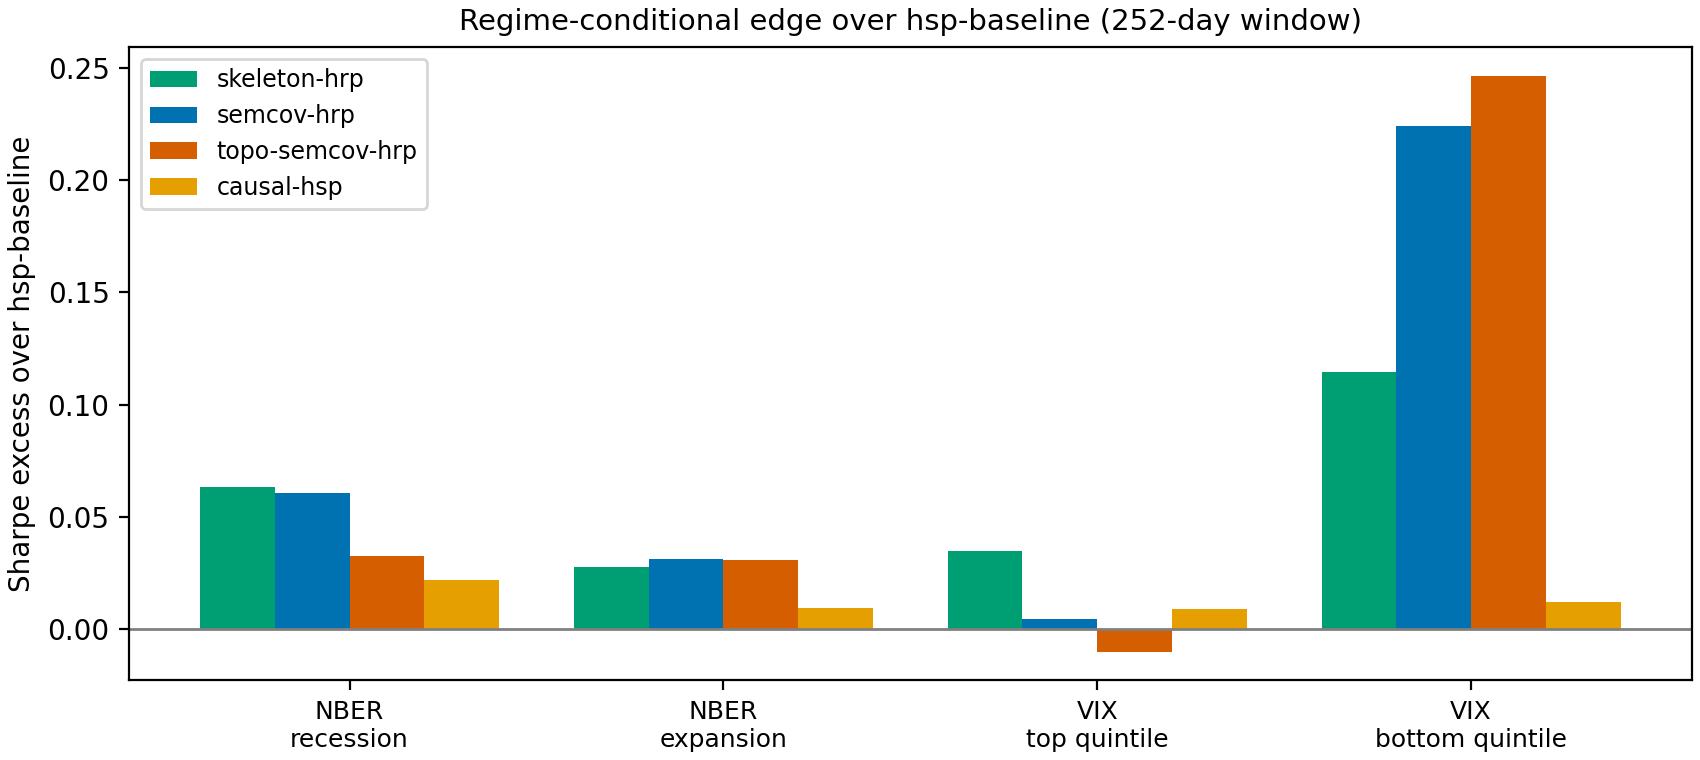
\includegraphics[width=0.9\textwidth]{figures/phase_ii_regime.png}
  \caption{Regime-conditional Sharpe excess over the \HRP{} control
    (one-year window).
    The
    orientation-aware edge concentrates in the VIX bottom quintile (calm
    markets), not in stress: the stress hypothesis is rejected.}
  \label{fig:regime}
\end{figure}

\begin{table}[h]
  \centering
  \caption{Regime-conditional annualised net Sharpe, window 252. High-vol
    and Low-vol are the top and bottom VIX quintiles; NBER columns condition
    on recession/expansion dates. Column-wise best in bold; the
    orientation-aware edge concentrates in the low-volatility regime.
    Conditional Sharpe levels are mechanically inflated in the calm
    regime (the volatility denominator conditions on low-VIX days); only
    within-column differences are meaningful.}
  \label{tab:regime-full}
  \begin{tabular}{l c c c c c}
    \toprule
    Variant & All & NBER rec. & NBER exp. & High-vol & Low-vol \\
    \midrule
    \HRP{}     & 0.381 & $-0.589$ & 0.737 & $\mathbf{-1.313}$ & 5.564 \\
    \skelsamp{} (skeleton)     & 0.403 & $\mathbf{-0.575}$ & 0.758 & $-1.317$ & 5.744 \\
    \skelsem{}                & \textbf{0.411} & $-0.577$ & \textbf{0.762} & $-1.347$ & 5.854 \\
    \orientsem{}               & 0.406 & $-0.606$ & 0.761 & $-1.361$ & \textbf{5.876} \\
    \bottomrule
  \end{tabular}
\end{table}

\section{The first phase: the driver route and its two null results}
\label{app:hsp}

The project's first phase built on Hierarchical Sensitivity Parity (HSP;
Section~\ref{sec:hrp-theme}) and asked whether replacing its
correlation-based driver selection with selection from a discovered causal
graph improves the allocation. Three configurations were evaluated on the
panel and protocol of Chapter~\ref{chap:evaluation}: HSP as published
(correlation-selected drivers, neural sensitivities, HRP on the sensitivity
distance); a causal-selection variant that chooses the $K{=}17$ drivers by
their aggregate outgoing influence in the DYNOTEARS graph (also run under
VARLiNGAM); and a closed-loop variant that feeds each month's realised
excess Sharpe over equal weight back into the driver scores through an
exponentially weighted utility with blend weight $\alpha$ and decay
$\gamma$. Over the one- and two-year windows, a sweep over
$K\in\{10,14,17,20,25\}$ and a $3\times3$ grid over $(\alpha,\gamma)$,
the phase contributes \rsNtrialsPhaseI\ of the \rsNtrials\ trials in the
deflation universe (two of them the skeleton cells that the replication
gate of Section~\ref{sec:ablation-design} targets); the remaining
\rsNtrialsPhaseII\ are the graph-route cells of this study. Both of the
phase's results were null.

\paragraph{The claimed improvement is inside the method's own noise.} At
the one-year window and $K{=}17$, causal selection beats HSP as published
by $+0.010$ net Sharpe ($p=0.27$); the sign reverses at $K=10$, $20$ and
$25$ ($-0.015$, $-0.016$, $-0.010$), and no difference at any $K$ is
significant ($p=0.10$--$0.77$). Re-running the identical causal-selection
configuration under \rsSeedN\ network seeds, with discovery cached so that
the initialisation is the only varying ingredient, moves its net Sharpe
across $[\rsSeedMin, \rsSeedMax]$ (median $\rsSeedMedian$;
Figure~\ref{fig:seed}). The seed
range ($\rsSeedRange$) is more than twice the $+0.010$ edge, and the
committed seed sits at the $\rsSeedPct$th percentile of its own
distribution, so at the least favourable seed the edge all but vanishes.
Plain correlation-distance HRP (\HRP{}) beats HSP as published at the same
window ($\rsCorrSharpe$ against $0.371$), so the driver-and-network
machinery subtracts value relative to textbook HRP, and the $90\%$ Model
Confidence Set over the \rsMcsUniverse\ distinct one-year strategies of
Section~\ref{sec:believe-rigour} retains \rsMcsSize\ of them and
eliminates only HSP as published. Every graph-route allocator of
Chapter~\ref{chap:sensitivity} is deterministic, and at the one-year window
each sits above the seed cloud's maximum.

\begin{figure}[tbp]
  \centering
  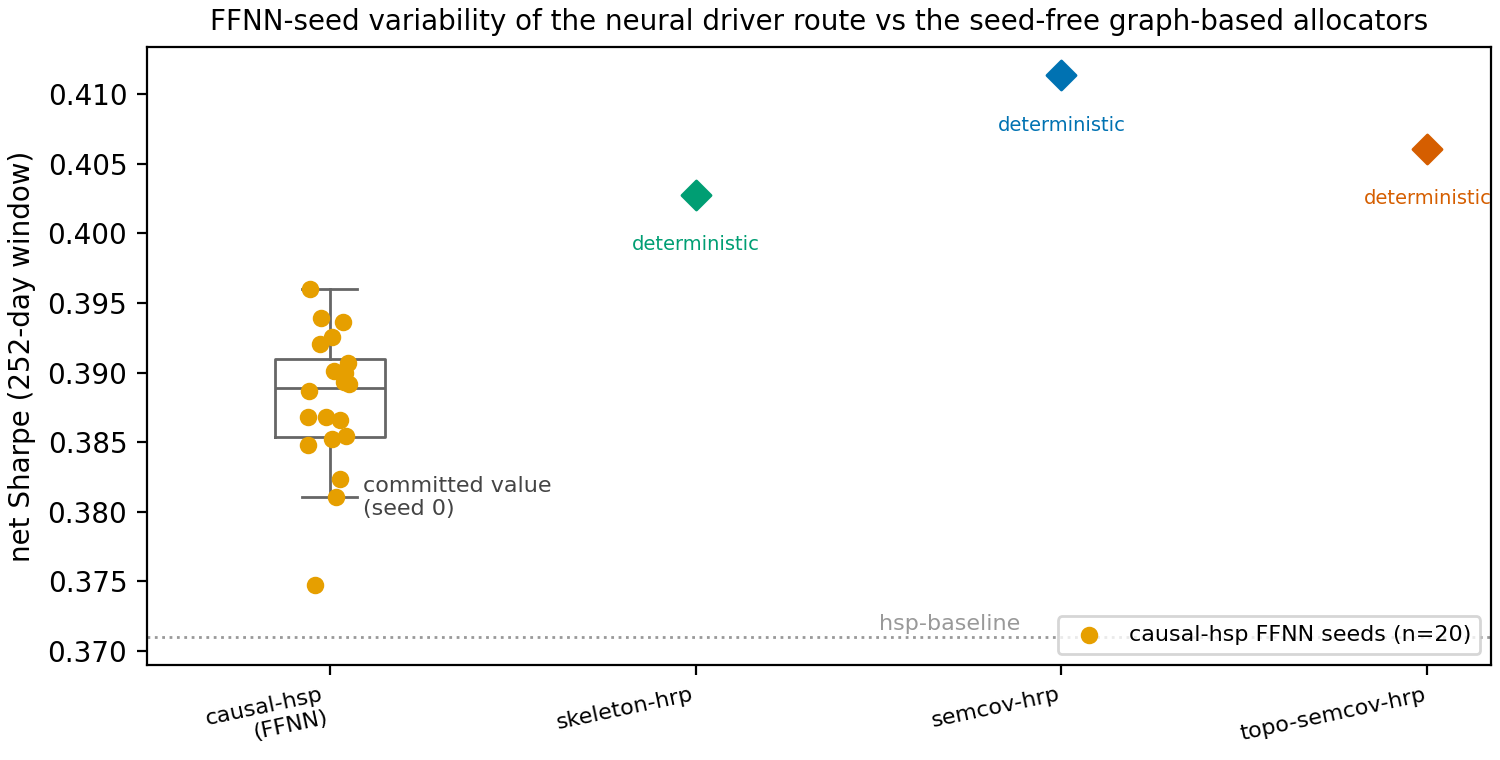
\includegraphics[width=0.85\textwidth]{figures/phase_ii_seed.png}
  \caption{The seed audit: net Sharpe of the causal-selection HSP variant
    across \rsSeedN\ network seeds at the one-year window, against HSP as
    published (dotted line) and the deterministic graph-route allocators
    of this study. The seed range exceeds the variant's claimed edge over
    its baseline, and every graph-route allocator shown sits above the
    seed cloud's maximum.}
  \label{fig:seed}
\end{figure}

\paragraph{The monthly feedback loop cannot learn.} Across the full
$\alpha\in\{0.4,0.6,0.8\}\times\gamma\in\{0.1,0.3,0.5\}$ grid the
closed loop's weights equal the open-loop variant's at every rebalance,
because the utility blend can only re-rank drivers within the causally
selected set. Even where it could act, its signal is too weak to act on:
the monthly reward is a Sharpe ratio estimated from 21 daily observations,
whose sampling standard error is about $\rsSharpeSE$, and across 215
rebalances it has mean $\rsRewardMean$ and standard deviation
$\rsRewardStd$, a per-update signal-to-noise ratio of about
$\rsRewardSNR$. A feedback rule at this frequency receives one number a
month that is almost entirely noise, so no learning rule could extract the
signal without lengthening the reward window or raising the update
frequency.

\section{Universe and driver lists}
\label{app:universe}

\paragraph{Asset universe (99 names).} AAPL, ABBV, ABT, ACN, ADBE, ADP,
AEP, AMGN, AMT, AMZN, AXP, BA, BAC, BKNG, BLK, BMY, C, CAT, CHTR, CI, CL,
CMCSA, COF, COP, COST, CRM, CSCO, CVS, CVX, D, DE, DHR, DIS, DUK, EBAY,
ED, EOG, ETN, EXC, F, FDX, GE, GILD, GIS, GM, GOOGL, GS, HD, HON, IBM,
INTC, JNJ, JPM, KMB, KO, LIN, LLY, LMT, LOW, MA, MCD, MDT, META, MMM, MO,
MRK, MS, MSFT, NEE, NKE, NVDA, ORCL, PEP, PFE, PG, PM, PNC, PSX, RTX,
SBUX, SCHW, SLB, SO, SPG, SRE, T, TFC, TGT, TMO, TMUS, TXN, UNH, UPS,
USB, V, VZ, WFC, WMT, XOM (tickers as of the CRSP mapping of
Section~\ref{sec:asset-graph}; the list is committed as
\texttt{scripts/phase\_i\_universe.txt}).

\paragraph{Driver pool (33 series).} Macro releases: CPI and core CPI
year-on-year, unemployment-rate change, industrial production
year-on-year, retail sales year-on-year, housing starts year-on-year,
Michigan sentiment change. Rates and spreads: 3-month, 2-, 5-, 10- and
30-year Treasury yield changes, 10y$-$2y and 10y$-$3m slope changes,
Baa$-$Aaa and Baa$-$10y credit-spread changes. Currencies: dollar-index
change; EURUSD, JPYUSD, GBPUSD and CNYUSD log returns. Commodities: WTI,
Brent, gold, natural gas, silver and copper log returns. Volatility and
international equity: VIX level; EFA, EEM, EWJ, EWG and EWU log returns.
(The catalogue's \texttt{hyg\_lqd\_logret} and \texttt{vvix} series are
excluded, as in the first phase.)

\section{Hyperparameters}

For reproducibility, the operative settings. Discovery: DYNOTEARS lag
$p=1$, $\lambda_W=\lambda_A=0.05$, fit-time edge threshold $0.01$ (the
extraction threshold $\tau$ of Section~\ref{sec:asset-graph} defaults to $0$
on top of this); VARLiNGAM with lingam pruning disabled (adaptive lasso
fails at $d>n$); ridge-Granger ridge $\lambda=10^{-2}$ scaled by window length,
density-matched per window to the paired DYNOTEARS graph.
Allocators: single-linkage where clustering is used;
$\Sigma_{\mathrm{SEM}}$ with diagonal shock variances from fit-window
residuals, nearest-PSD projection and ridge load
$10^{-6}\operatorname{tr}(\Sigma)/N$; topological tie-break by
total downstream influence then name.
Protocol: 5\,bps one-way (swept $\{0,5,10,20\}$); windows
189/252/378/504 trading days; holding and step 21 trading days; 215
(189- and 252-day windows) / 209 (378-day) / 203 (504-day) rebalances,
2007-01--2024-11
(shorter-lookback rebalances before a window's burn-in completes fall back
to equal weight, identically for every allocator at that window);
Politis--Romano bootstrap, 10{,}000 resamples, mean block 21 trading days.

\section{Reproducibility}

All results derive from committed code and cached data and are
exactly reproducible: after the data-determinism fix of
Section~\ref{sec:cache},
two independent end-to-end runs produce identical graphs, weights and
NAVs, verified by the replication gate (\skelsamp{} vs the prior phase's committed
bundle: $\Delta$Sharpe $= 0$, max weight difference $= 0.0$ over all 215
rebalances; re-verified on the four-window grid by an exact repeat
of a 378-day cell). The ablation ran on 1{,}684 cache-verified graph fits
with a 100\% hit rate; each backtest regenerates in ${\approx}40$ seconds
from the cache.

\paragraph{Cache mechanics and the determinism defect.} The discovery
cache is keyed by the exact window bytes, column set, method and
hyperparameters, with atomic writes; a key miss halts the run rather
than silently refitting a subtly different graph. The data-determinism
defect of Section~\ref{sec:cache} arose because EEM's 2003 inception
fell inside the cache-coverage check's padding window, triggering a
silent re-download whose auto-adjustment jittered values by
${\approx}3\times10^{-7}$ run-to-run; the non-convex DYNOTEARS
optimiser amplified this into graph changes of ${\approx}0.14$ in
$\lVert W\rVert$, while VARLiNGAM's ICA-on-residuals fits were
essentially unchanged by the same jitter, a small robustness result in
its own right.

\paragraph{Environment and data access.} Python~3.13 in the repository's
virtual environment; \texttt{causalnex} and \texttt{lingam} are vendored
(source-tree imports via \texttt{\_vendored.py}), not pip-installed, so
their exact versions are pinned by the repository itself. All commands run
from the repository root, from which \texttt{pipeline} imports as a package.
Raw market data requires a WRDS/CRSP licence; the fitted graphs and derived
series are committed to the content-keyed cache, so every result in this
report regenerates offline without it.

\paragraph{Regeneration order.} An informed reader reproduces the report in
four steps, each idempotent against the cache: (1) run the unit-test suite
(60+ tests, including the orientation-blindness and orientation-sensitivity
properties of Section~\ref{sec:ablation-design}); (2) run the backtest grid,
which verifies every graph fit as a cache hit (a miss halts the run
rather than silently refitting); (3) rebuild the statistics macros with
\texttt{scripts/robust\_stats.py -{}-phase-ii}; (4) rebuild the figures with
\texttt{scripts/plot\_phase\_ii\_figures.py} and compile the report.
\paragraph{Provenance.} Every statistic quoted in the text is either a
generated macro (\path{_generated/robust_stats.tex}) or traceable to a
committed CSV (\path{results/phase_ii_matrix.csv},
\path{phase_ii_contrasts.csv}, \path{robust_stats_phase_ii.csv},
\path{regime_analysis/},
\path{oos_slice.csv}/\path{oos_contrasts.csv}); every figure is
regenerated by the plotting script above. No result in the 2007--2024
panel depends on a live network fetch.

\paragraph{The out-of-sample slice.} The 2025--26 slice of
Section~\ref{sec:oos} is regenerated by
\texttt{scripts/run\_oos\_slice.py} (per allocator and window) followed
by \texttt{scripts/collate\_oos.py}. Its protocol, price-source rule
and outcome interpretations were committed in advance in
\texttt{PREDICTIONS\_OOS.md}. The slice keeps its own price and driver
caches (\path{cache/prices_oos}, \path{cache/drivers_oos}) so the
2007--2024 CRSP caches are never rewritten, and its asset prices come
from Yahoo Finance because CRSP daily data ends 2024-12-31 (verified
against WRDS on 2026-08-15); its DYNOTEARS fits join the shared
content-keyed discovery cache under their own keys.

\end{document}
